\chapter{Diseño e implementación} % Main chapter title

\label{Chapter3} % Change X to a consecutive number; for referencing this chapter elsewhere, use \ref{ChapterX}

\definecolor{mygreen}{rgb}{0,0.6,0}
\definecolor{mygray}{rgb}{0.5,0.5,0.5}
\definecolor{mymauve}{rgb}{0.58,0,0.82}

%%%%%%%%%%%%%%%%%%%%%%%%%%%%%%%%%%%%%%%%%%%%%%%%%%%%%%%%%%%%%%%%%%%%%%%%%%%%%
% parámetros para configurar el formato del código en los entornos lstlisting
%%%%%%%%%%%%%%%%%%%%%%%%%%%%%%%%%%%%%%%%%%%%%%%%%%%%%%%%%%%%%%%%%%%%%%%%%%%%%
\lstset{ %
  backgroundcolor=\color{white},   % choose the background color; you must add \usepackage{color} or \usepackage{xcolor}
  basicstyle=\footnotesize,        % the size of the fonts that are used for the code
  breakatwhitespace=false,         % sets if automatic breaks should only happen at whitespace
  breaklines=true,                 % sets automatic line breaking
  captionpos=b,                    % sets the caption-position to bottom
  commentstyle=\color{mygreen},    % comment style
  deletekeywords={...},            % if you want to delete keywords from the given language
  %escapeinside={\%*}{*)},          % if you want to add LaTeX within your code
  %extendedchars=true,              % lets you use non-ASCII characters; for 8-bits encodings only, does not work with UTF-8
  %frame=single,	                % adds a frame around the code
  keepspaces=true,                 % keeps spaces in text, useful for keeping indentation of code (possibly needs columns=flexible)
  keywordstyle=\color{blue},       % keyword style
  language=[ANSI]C,                % the language of the code
  %otherkeywords={*,...},           % if you want to add more keywords to the set
  numbers=left,                    % where to put the line-numbers; possible values are (none, left, right)
  numbersep=5pt,                   % how far the line-numbers are from the code
  numberstyle=\tiny\color{mygray}, % the style that is used for the line-numbers
  rulecolor=\color{black},         % if not set, the frame-color may be changed on line-breaks within not-black text (e.g. comments (green here))
  showspaces=false,                % show spaces everywhere adding particular underscores; it overrides 'showstringspaces'
  showstringspaces=false,          % underline spaces within strings only
  showtabs=false,                  % show tabs within strings adding particular underscores
  stepnumber=1,                    % the step between two line-numbers. If it's 1, each line will be numbered
  stringstyle=\color{mymauve},     % string literal style
  tabsize=2,	                   % sets default tabsize to 2 spaces
  title=\lstname,                  % show the filename of files included with \lstinputlisting; also try caption instead of title
  morecomment=[s]{/*}{*/}
}


%----------------------------------------------------------------------------------------
%	SECTION 1
%----------------------------------------------------------------------------------------
\section{Arquitectura general del sistema}
\label{sec:arquitecturagral}

\subsection{Funcionamiento}
\label{subsec:funcionamiento}
Como se puede observar en la figura \ref{fig:diagramafunciones}, el sistema está compuesto por nodos, los cuales se utilizan para la lectura de tarjetas RFID asignadas a los repuestos de los clientes. Los datos se transmiten en una red local, se procesan y almacenan en un servidor con base de datos y son consultados desde la aplicación web en las terminales (\textit{PC} o \textit{smartphone}).

\begin{figure}[H]
	\centering
	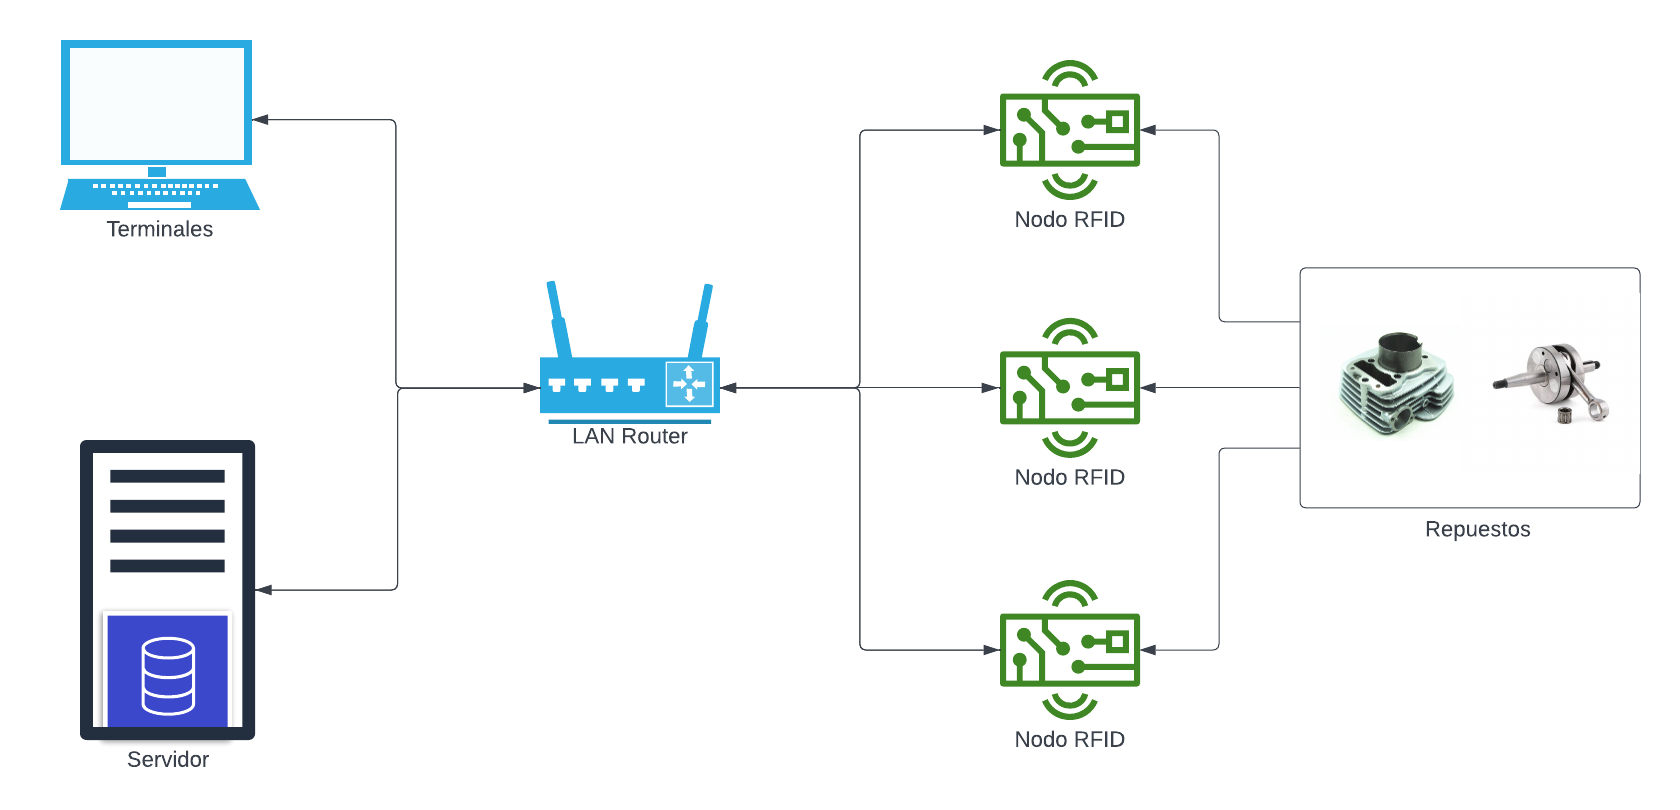
\includegraphics[scale=.50]{./Figures/diagramafunciones.png}
	\caption{Diagrama de funciones generales.}
	\label{fig:diagramafunciones}
\end{figure}

\subsection{Diagrama de bloques}
\label{subsec:diagramabloques}
En la figura \ref{fig:diagramabloques} se representa el patrón de modelo conceptual empleado y las tecnologías que se utilizan en cada capa. Se implementó un modelo de 4 capas: 

\begin{itemize}
\item Capa de percepción.
\item Capa de transporte.
\item Capa de procesamiento.
\item Capa de aplicación.
\end{itemize}


\begin{figure}[H]
	\centering
	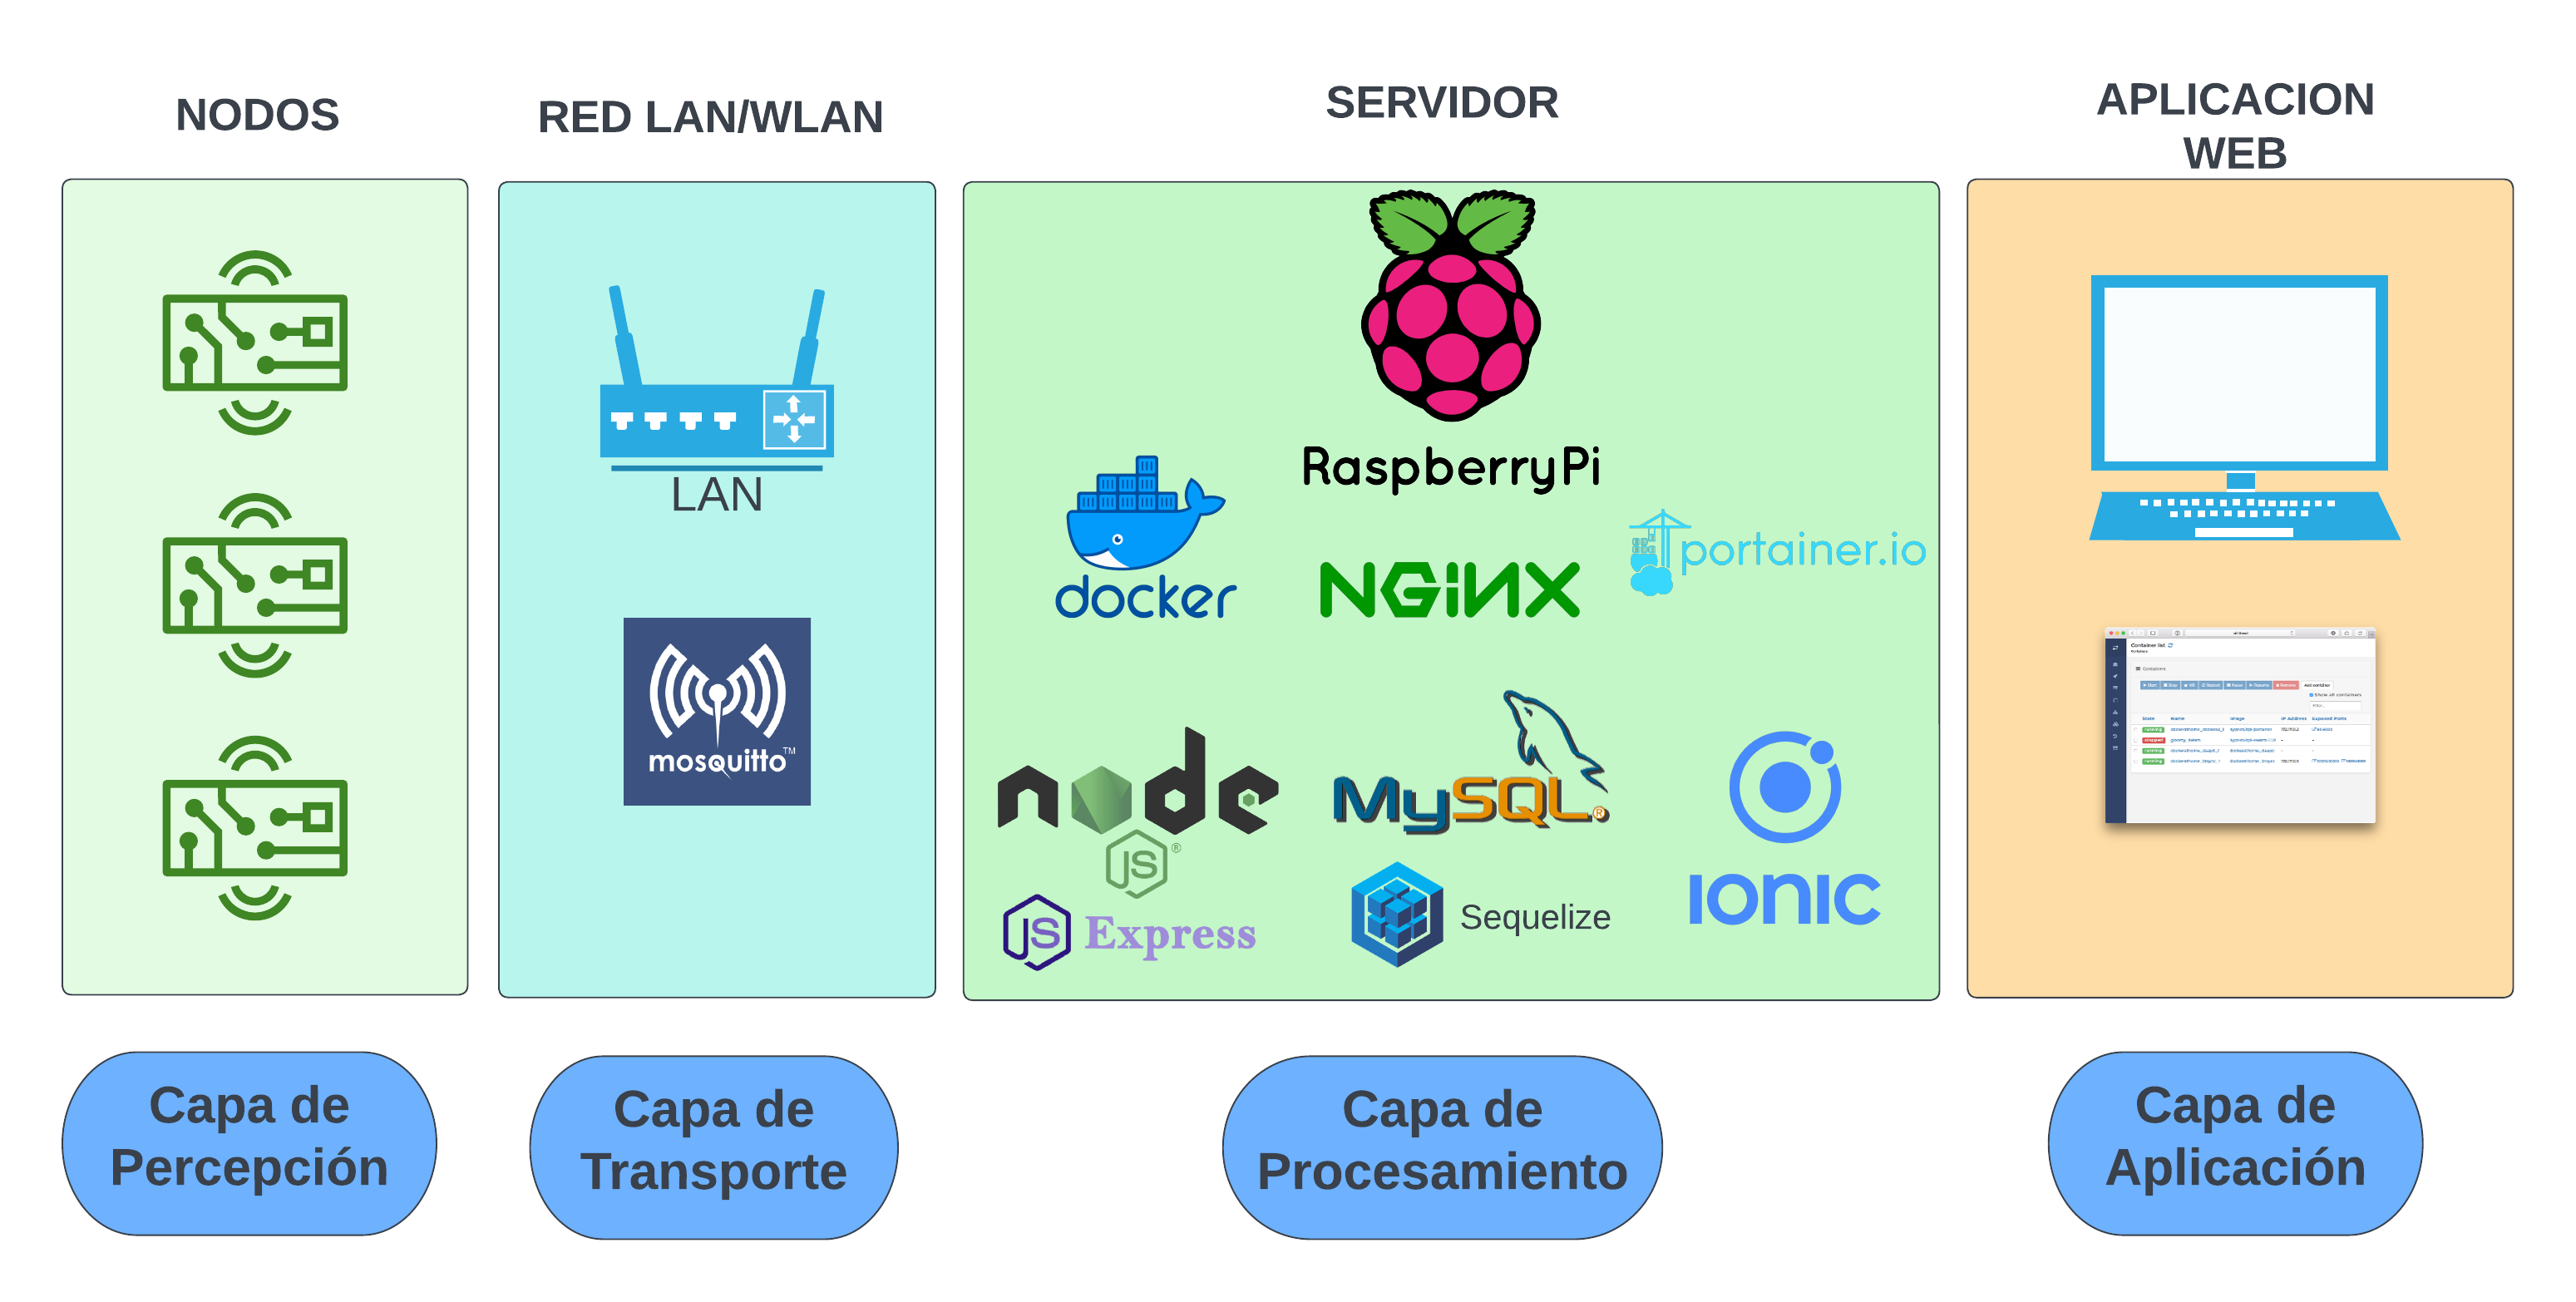
\includegraphics[scale=.25]{./Figures/diagramabloques.png}
	\caption{Diagrama de bloques y tecnologías del sistema.}
	\label{fig:diagramabloques}
\end{figure}


En la capa de percepción se utilizan los nodos ESP32 con lector RFID con los cuales se realiza la lectura de las tarjetas correspondientes. Una vez realizada la lectura, los datos son enviados por medio del protocolo MQTT y a través de la red local en la capa de transporte. 

La capa de transporte es la encargada de transmitir los mensajes por medio de los protocolos MQTT y HTTP. El \textit{broker} Eclipse Mosquitto distribuye los mensajes publicados a los suscriptores para su procesamiento.

En la capa de procesamiento se realiza la lógica del \textit{backend}, la base de datos y el \textit{frontend}. Se implementó un servidor central en una Raspberry Pi 4 con todos los servicios. Cada uno de los servicios está desarrollado de manera individual y fue montado en su propio contenedor de Docker. Todos los contenedores se despliegan utilizando Docker Compose.

Por último, la capa de aplicación otorga el acceso web, desarrollado en el \textit{framework } \textit{Ionic}, para el ingreso, registro, administración y egreso de las órdenes de trabajo. También se utiliza el portal de administración de \textit{Portainer} para el monitoreo completo de Docker y del servidor.


\section{Flujo general del sistema}
\label{sec:flujogeneral}
En esta sección se explica el flujo total de las funciones del sistema desde que el usuario ingresa una nueva órden de trabajo hasta que el producto es retirado por el cliente.

Las comunicaciones y el envío de datos entre los distintos módulos del sistema se realizan en los protocolos HTTP, MQTT y MySQL. Se detallará en cada caso el protocolo utilizado.

\subsection{Ingreso de repuesto}
\label{subsec:ingresorepuesto}
En la figura \ref{fig:flujoingreso} se puede observar todos los módulos del sistema, el flujo de datos y protocolos que intervienen cuando un usuario carga una nueva órden de trabajo en el sistema.

\begin{figure}[ht]
	\centering
	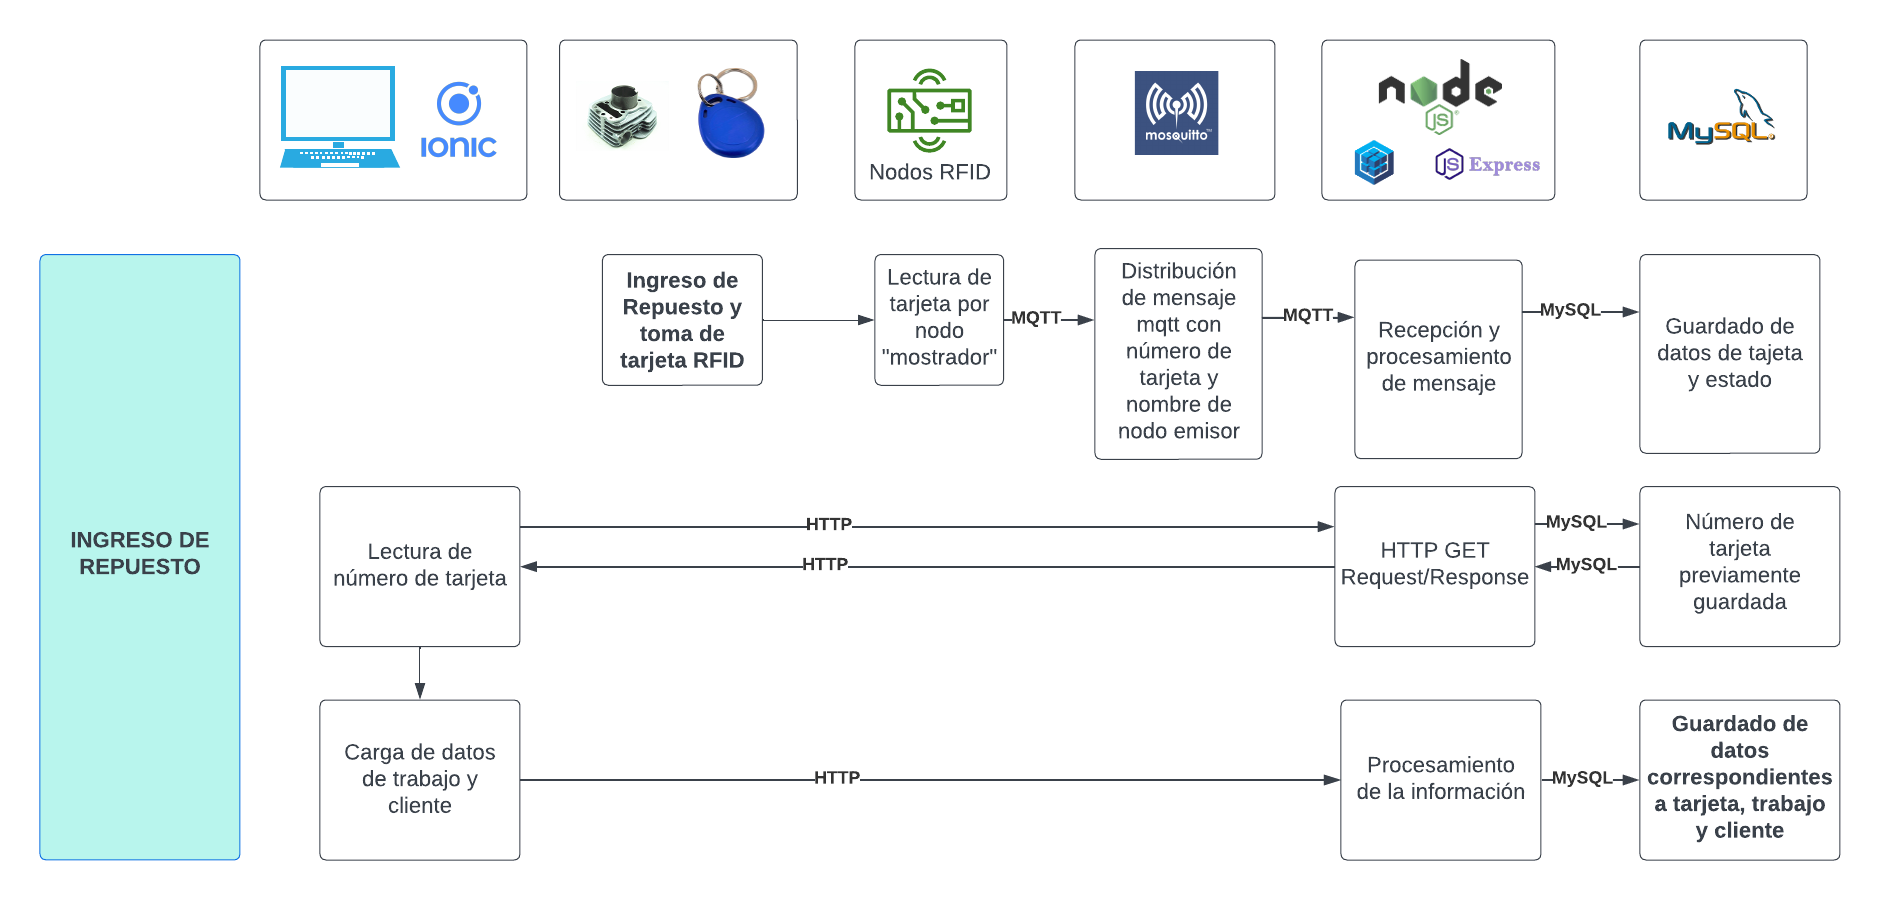
\includegraphics[scale=.20]{./Figures/flujoingreso.png}
	\caption{Flujo en el ingreso de una nueva órden de trabajo.}
	\label{fig:flujoingreso}
\end{figure}
  
El flujo inicia cuando el usuario recibe el repuesto y selecciona una tarjeta RFID libre para usarla con ese repuesto. El usuario pasa la tarjeta por el nodo ubicado en la recepción, nodo \textit{mostrador}, y de esta manera se registra el número de tarjeta para ser utilizada. Luego el usuario carga los datos en la aplicación web, dónde ya está asignada la tarjeta previamente leída, confirma los datos y estos son guardados en la base de datos. La nueva órden de trabajo tiene su número de tarjeta, los datos del cliente y el estado por defecto \textit{en espera}.

\subsection{Cambio de estado}
\label{subsec:flujocambioestado}

En la figura \ref{fig:flujocambioestado} podemos observar el flujo completo para un cambio de estado de una órden de trabajo.

\begin{figure}[ht]
	\centering
	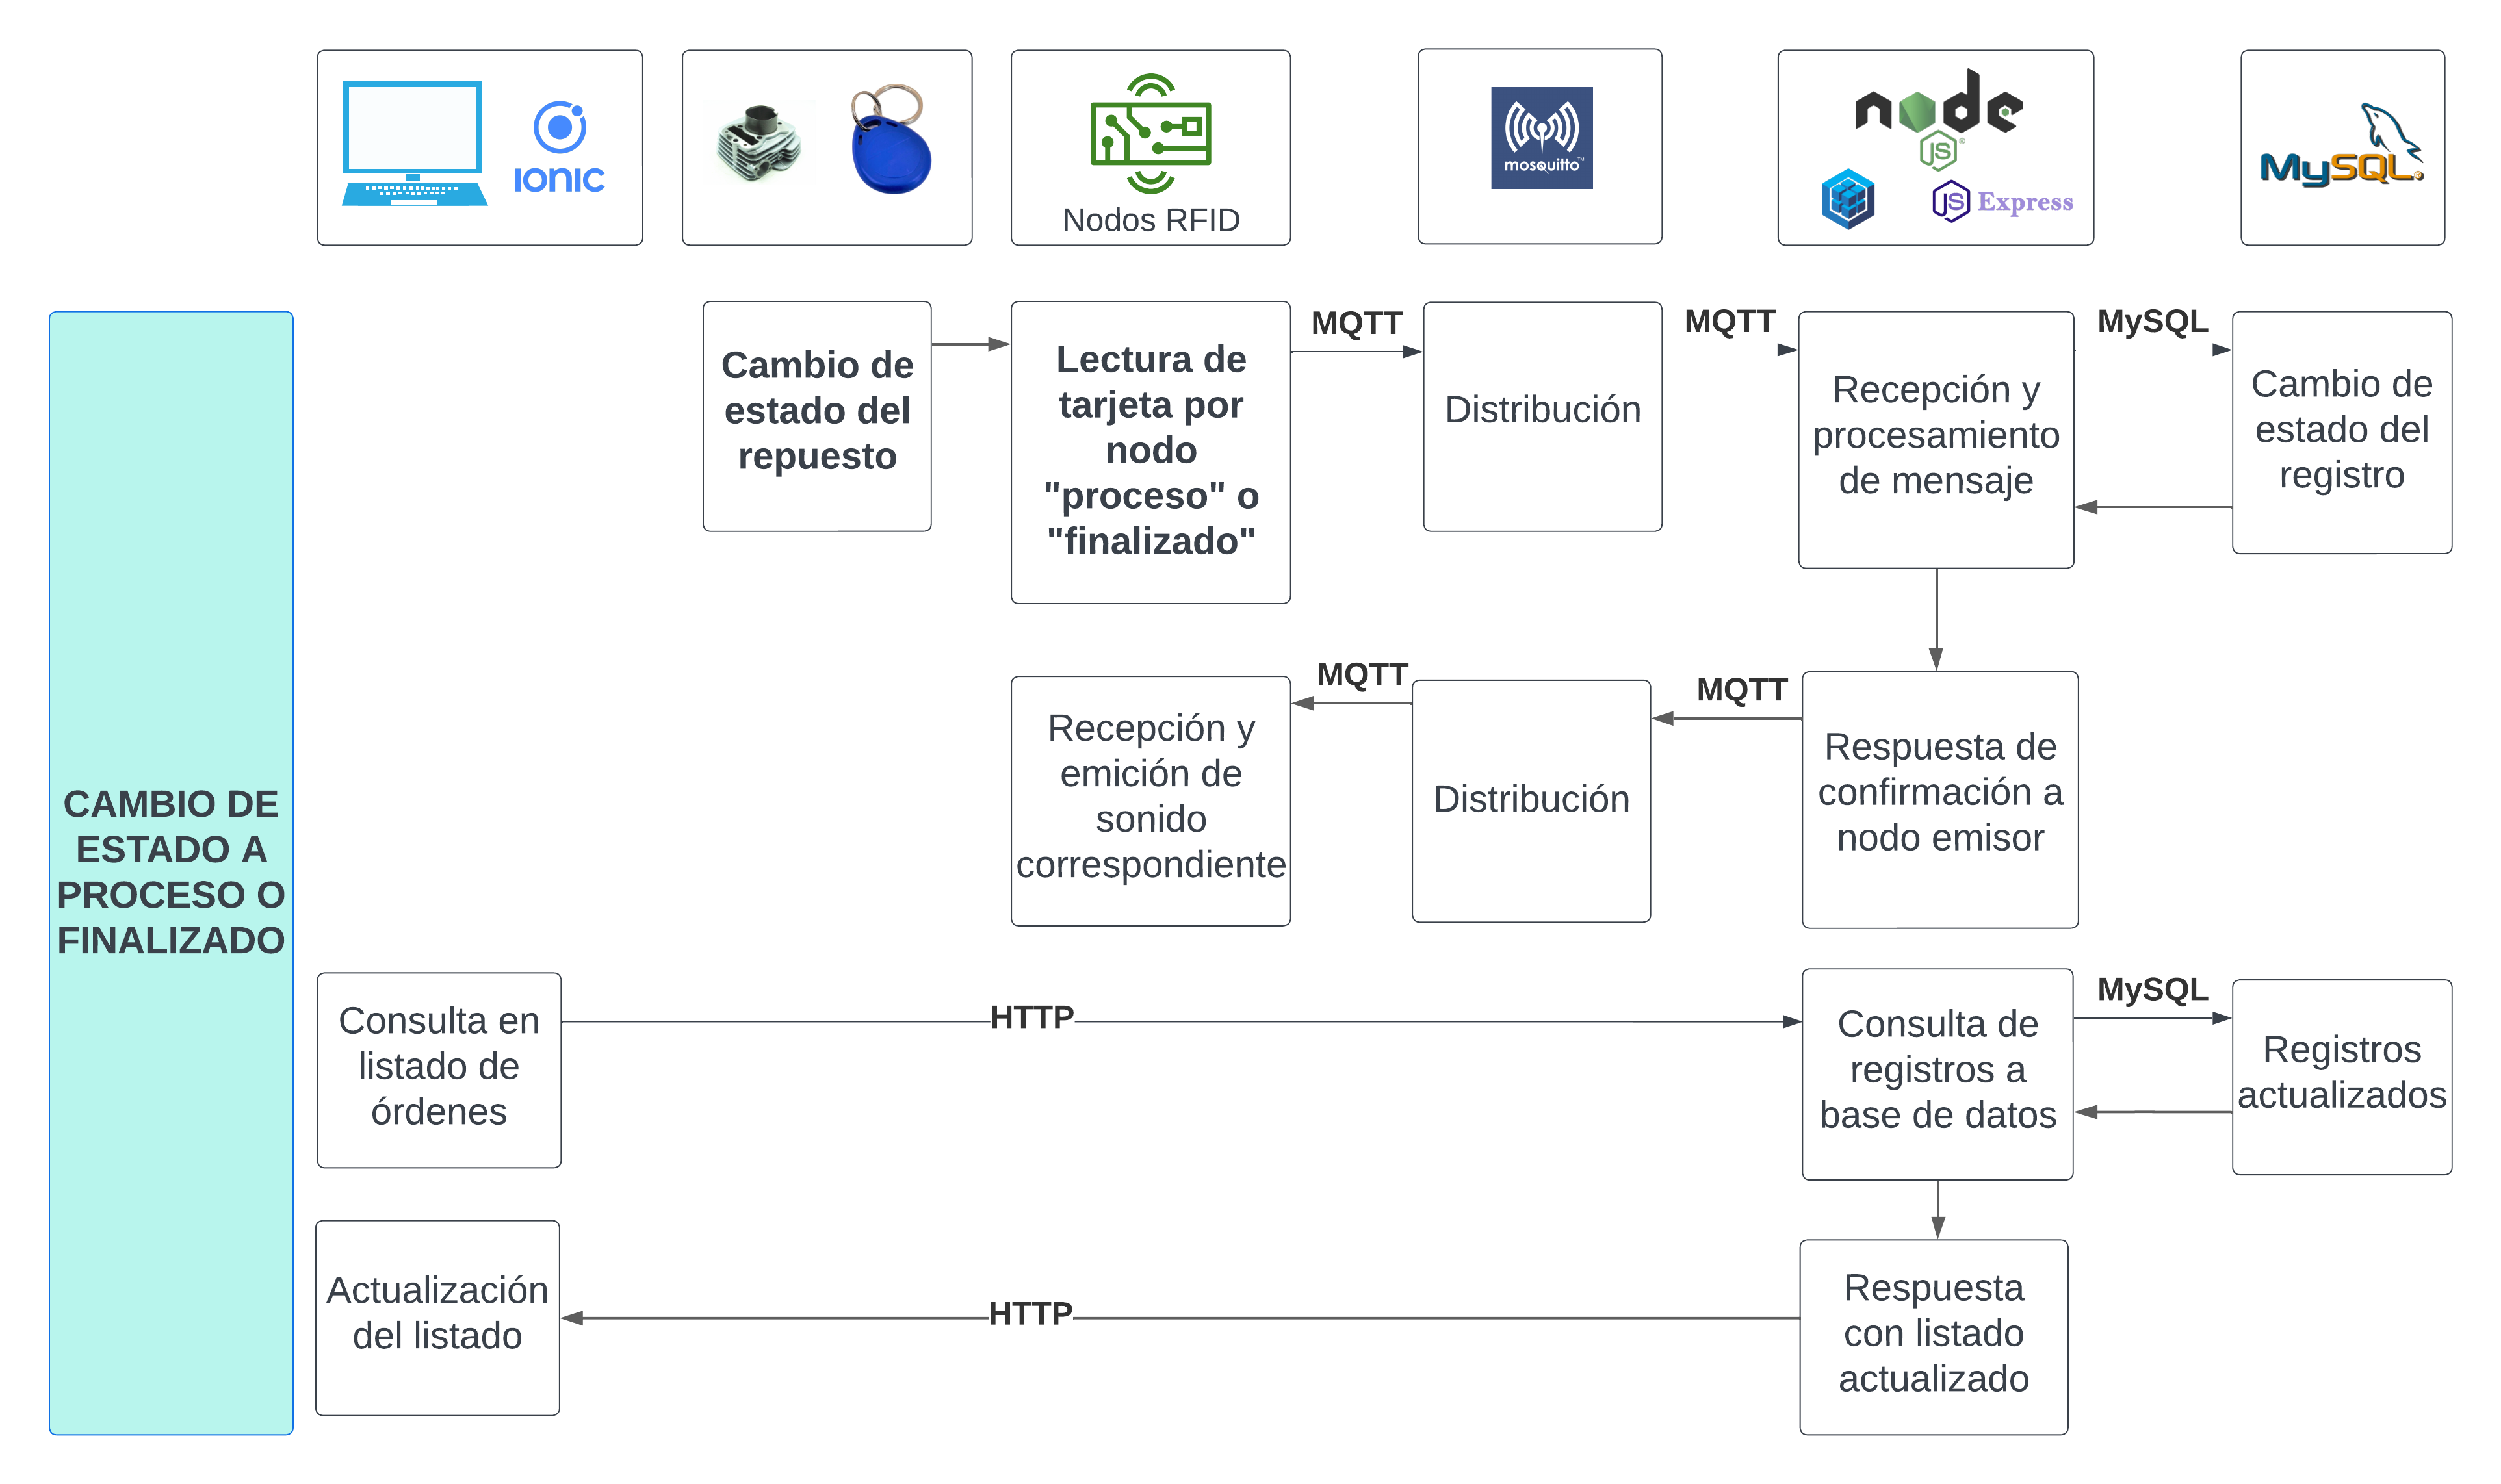
\includegraphics[scale=.10]{./Figures/flujo-cambio-estado.png}
	\caption{Flujo en el cambio de estado de una órden de trabajo.}
	\label{fig:flujocambioestado}
\end{figure}

El flujo inicia cuando un trabajador inicia o finaliza una óden, cambiando el estado de la misma a \textit{en proceso} o \textit{finalizada}. Para actualizar el estado de la órden debe pasar la tarjeta RFID asociada al repuesto por el nodo correspondiente, de esta manera se transmite la información por protocolo MQTT hasta la API de \textit{backend}, esta última realiza el la actualización en la base de datos y responde al nodo por medio de MQTT informando si la operación tuvo éxito. El nodo emitirá un sonido que informará al usuario del resultado obtenido (tabla de sonidos en capítulo \ref{subsec:mqttnodos}). Al mismo tiempo el usuario de la aplicación web verá reflejada la actualización del estado de la órden correspondiente en el listado de órdenes, ya que se está constantemente consultando por actualizaciones a la API por medio del protocolo HTTP utilizando el patrón observador de IONIC (detallado en el capítulo \ref{subsec:frontinterfaces}).

\subsection{Retiro de repuesto}
\label{subsec:flujoretiro}

En la figura \ref{fig:flujoretiro} podemos observar el flujo completo en el retiro de un repuesto.

\begin{figure}[ht]
	\centering
	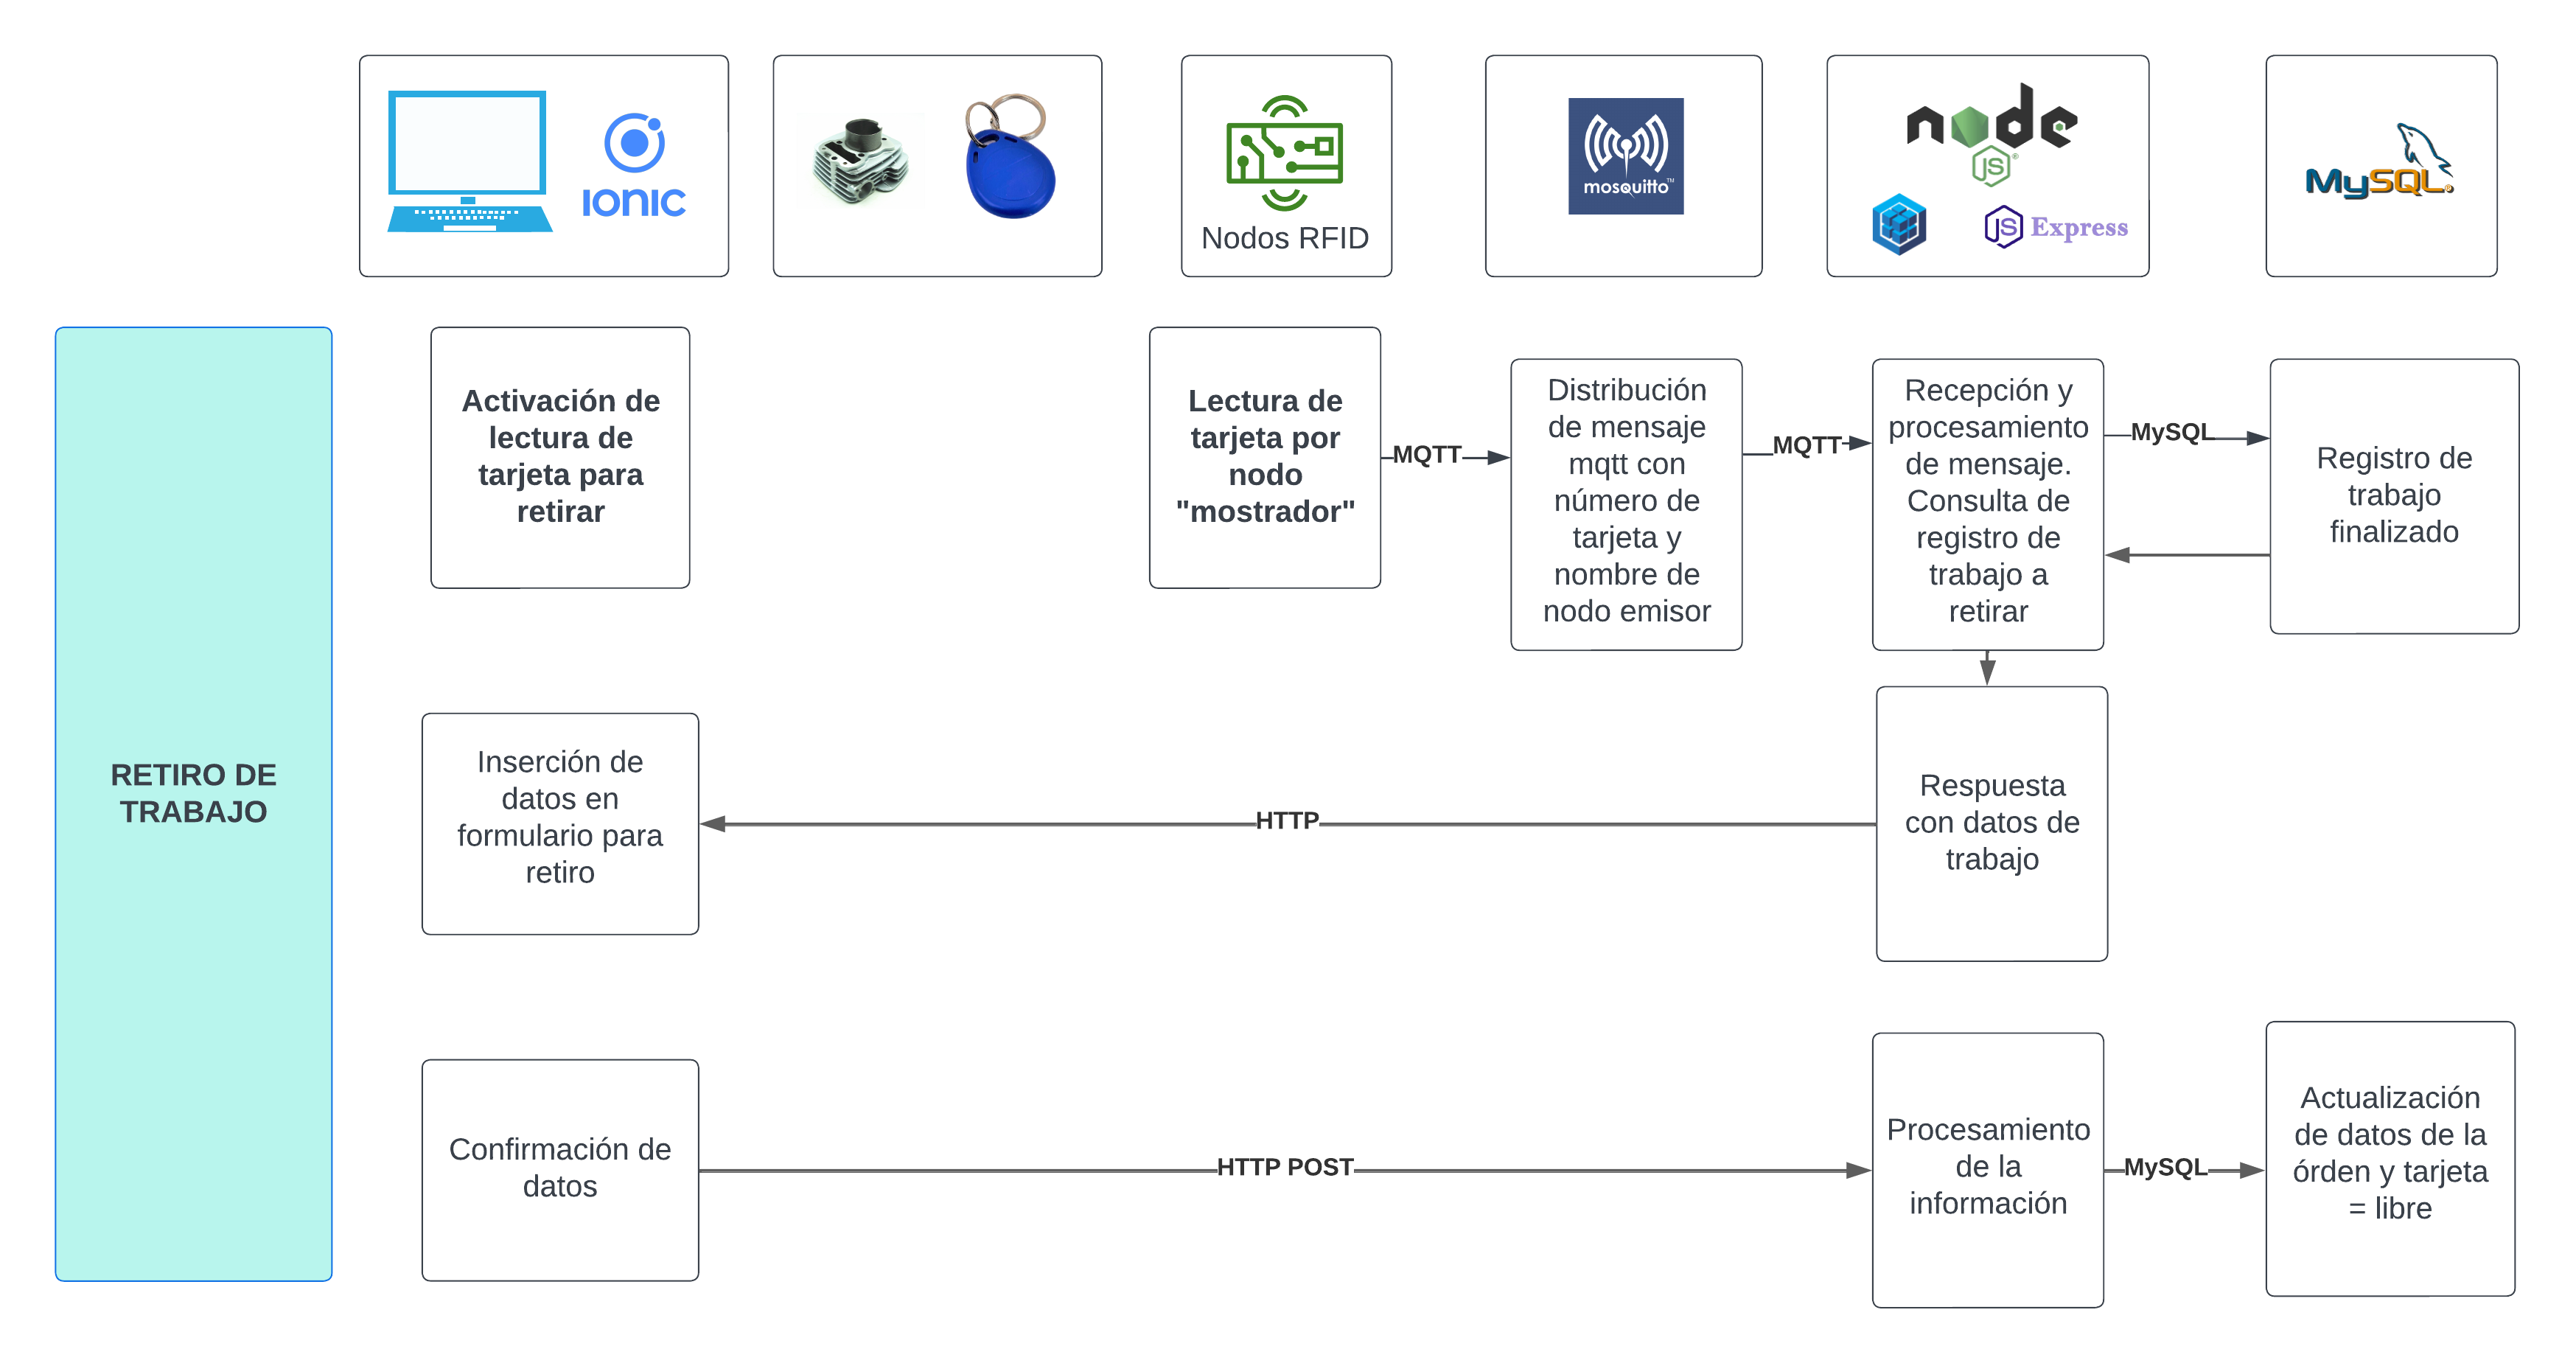
\includegraphics[scale=.10]{./Figures/flujo-retiro.png}
	\caption{Flujo en el retiro de una órden de trabajo.}
	\label{fig:flujoretiro}
\end{figure}

El flujo inicia cuando el usuario de la aplicación web realiza una activación de lectura de tarjeta en la pantalla de retiro. Esto ocasiona que la aplicación active un \textit{modo escucha} hacia la API, esperando a que el usuario pase la tarjeta asociada al repuesto por el nodo \textit{mostrador}. Cuando esto sucede la API recibe por MQTT el número de tarjeta y mediante este recupera los datos de la órden correspondiente en la base de datos, luego devuelve los datos obtenidos a la aplicación web por medio del protocolo HTTP. La aplicación inserta todos estos datos en el formulario de retiro y, cuando el usuario confirma la operación, se realiza una petición HTTP con el método PUT para actualizar los datos de los registros. La tarjeta utilizada queda en estado \textit{libre} para ser reutilizada en una nueva órden de trabajo.

\section{Arquitectura de datos}
\label{sec:arquitecturadatos}
En la presente sección se desarrollará la arquitectura en la base de datos MySQL, el diseño y la implementación de las funciones con el ORM Sequelize.

\subsection{Diagrama de base de datos}
\label{subsec:diagramabasededatos}

En la figura \ref{fig:diagramabbdd} se representa un diagrama UML de la base de datos con sus tablas y relaciones.

Para realizar el diseño de la base de datos se realizó un análisis de los requerimientos y los casos de usos o historias de usuario, a partir de esto se inició el diagrama con las tablas principales y sus relaciones, a medida que se avanzaba en el desarrollo de la API y del sistema  se fueron añadiendo nuevas tablas y relaciones según las necesidades. 

\begin{figure}[h]
	\centering
	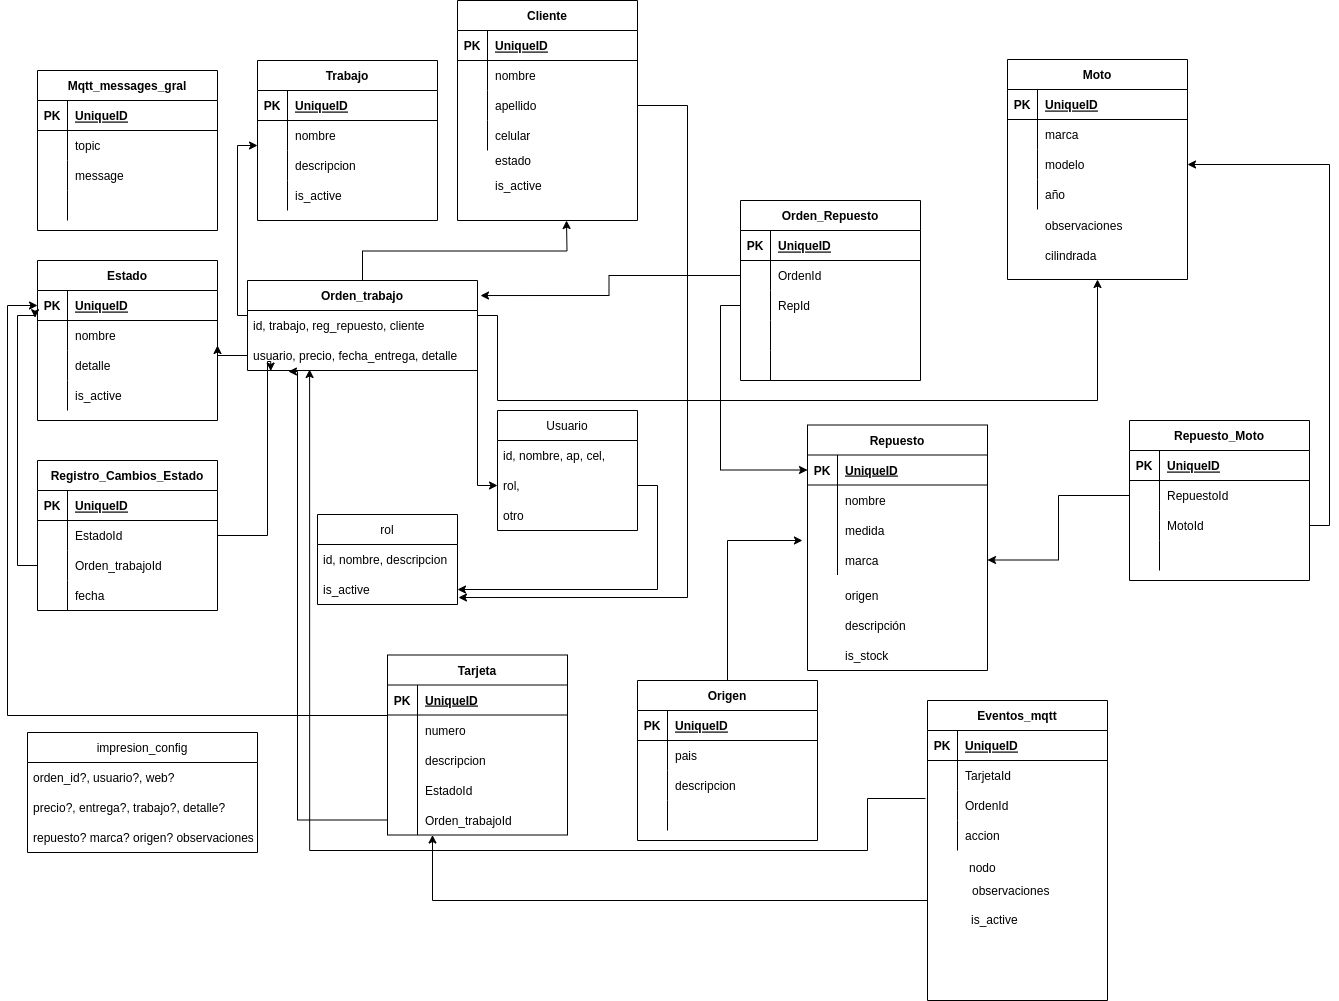
\includegraphics[scale=.27]{./Figures/diagramabbdd.png}
	\caption{Diagrama de base de datos.}
	\label{fig:diagramabbdd}
\end{figure}

\subsection{Estructura de archivos para ORM}
\label{subsec:estructuraorm}
Para el desarrollo de la base de datos se utilizó el ORM Sequelize. Como se menciona en el capítulo \ref{subsec:sequelize}, existen múltiples ventajas al utilizar un ORM en vez de directamente programar la base de datos en lenguaje SQL, se tuvieron en cuenta esas ventajas a la hora de optar por realizar el desarrollo con este ORM. 

La estructura de carpetas y archivos está definida previamente por el ORM pudiendo realizar algunas personalizaciones. 

En la figura \ref{fig:estructuraorm} podemos ver la estructura implementada.

\begin{figure}[h]
	\centering
	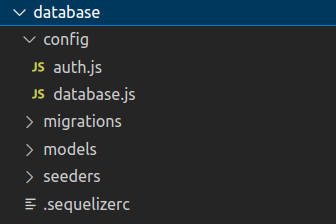
\includegraphics[scale=.50]{./Figures/estructuraorm.png}
	\caption{Estructura de carpetas y archivos para ORM Sequelize.}
	\label{fig:estructuraorm}
\end{figure}

Dentro de la carpeta \textit{config} se definen los archivos de configuración de Sequelize y el acceso a la base de datos MySQL.

En la carpeta migrations, models y seeders se encuentran todos los archivos Javascript para las migraciones, los modelos y semillas, estos archivos se detallarán en las próximas secciones. 

El archivo \textit{.sequelizerc} sirve para definir la ubicación de los modelos, migraciones, semillas y otros archivos generados por Sequelize.


\subsection{Desarrollo de modelos y tablas}
\label{subsec:modelobasededatos}



A continuación se presentan algunos fragmentos de código fuente empleados para el desarrollo de la base de datos, siguiendo esta misma modalidad se realizaron todas las tablas de la base de datos, sus modificaciones y sus respectivas migraciones.


El siguiente código se ejecuta en la terminal de linux para crear el archivo para el modelo y el archivo para la migración de la tabla para ``Órden de trabajo". En el código se define el nombre del modelo y un atributo id. 

\begin{lstlisting}[label=cod:sequelizeclimodel,caption=Código CLI para crear modelo y migración en Sequelize.]
npx sequelize-cli model:generate --name mqtt_messages_gral --attributes id:integer
\end{lstlisting}

El siguiente código se emplea para definir el modelo completo de la tabla:

\begin{lstlisting}[caption= Código para un modelo en Sequelize.]
'use strict';
const {Model} = require('sequelize');
module.exports = (sequelize, DataTypes) => {
  class OrdenTrabajo extends Model {
    
    static associate(models) {
      //OrdenTrabajo.X pertenece a X
      OrdenTrabajo.belongsTo(models.Trabajo)
      OrdenTrabajo.belongsTo(models.Estado)
      OrdenTrabajo.belongsTo(models.Cliente)
      OrdenTrabajo.belongsTo(models.Usuario)
      OrdenTrabajo.belongsTo(models.Moto)

      //OrdenTrabajo tiene ids en la tabla Eventos_mqtt
      OrdenTrabajo.hasMany(models.Eventos_mqtt);

      //OrdenTrabajo tiene id en la tabla Tarjeta
      OrdenTrabajo.hasMany(models.Tarjeta);

      // Orden_trabjo tiene muchos Cambios de Estado N:M
      OrdenTrabajo.belongsToMany(models.Estado, {
        through: 'Registo_cambios_estado'
      })

      // Orden de trabajo tiene muchos Repuestos N:M
      OrdenTrabajo.belongsToMany(models.Repuesto, {
        through: 'Orden_Repuesto'
      })


    }
  }
  OrdenTrabajo.init({
    id: {
      allowNull: false,
      autoIncrement: true,
      primaryKey: true,
      type: DataTypes.INTEGER
    },
    precio:{
      type: DataTypes.INTEGER
    },
    entrega:{
      type: DataTypes.INTEGER
    },
    fecha_entrega_estimada:{
      type: DataTypes.DATE
    },
    detalle:{
      type: DataTypes.TEXT('long')
    },
    tarjeta:{
      type: DataTypes.STRING
    },
    ordenPapel:{
      type: DataTypes.STRING
    },
    informado:{
      type: DataTypes.BOOLEAN
    },
    is_active: {
      type: DataTypes.BOOLEAN
    },
    createdAt: {
      allowNull: false,
      type: DataTypes.DATE
    },
    updatedAt: {
      allowNull: false,
      type: DataTypes.DATE
    }
  }, {
    sequelize,
    modelName: 'OrdenTrabajo',
    tableName: 'OrdenTrabajo',
  });
  return OrdenTrabajo;
};

\end{lstlisting}

En las líneas 1 a la 4 se realizan las declaraciones de la librería y el nombre del modelo, 
luego en las líneas 6 a la 31 se definen las relaciones que tendrá el modelo, los tipos de relaciones pueden ser 1 a 1, 1 a muchos o muchos a muchos. Luego a partir de la línea 33 se definen los campos de la tabla o modelo, se definen también los atributos de los campos y el tipo de datos. En las líneas 74 y 75 se define el nombre personalizado que tendrá la tabla en la base de datos y el nombre del modelo que reconocerá el ORM. Por último en la línea 77 se retorna la Clase creada, de esta manera podrá ser utilizada en otras partes del código fuente.


\subsection{Desarrollo de migraciones}
\label{subsec:migracionesbasededatos}

Como se menciona en la sección anterior, el archivo con la estructura inicial de migraciones se crea a través del CLI de Sequelize al momento de crear el modelo para una tabla, luego hay que personalizar esta estructura para que quede igual al modelo definido previamente. 

A continuación se representa el código \textit{javascript} para la migración del modelo ``Órden de trabajo":

\begin{lstlisting}[caption= Código para migración en Sequelize.]
'use strict';
module.exports = {
  async up(queryInterface, Sequelize) {
    await queryInterface.createTable('OrdenTrabajo', {
      id: {
        allowNull: false,
        autoIncrement: true,
        primaryKey: true,
        type: Sequelize.INTEGER
      },
      nombre: {
        type: Sequelize.STRING
      },
      precio:{
        type: Sequelize.INTEGER
      },
      entrega:{
        type: Sequelize.INTEGER
      },
      fecha_entrega_estimada:{
        type: Sequelize.DATE
      },
      detalle:{
        type: Sequelize.TEXT('long')
      },
      tarjeta:{
        type: Sequelize.STRING
      },
      ordenPapel:{
        type: Sequelize.STRING
      },
      informado:{
        type: Sequelize.BOOLEAN,
        defaultValue:false
      },
      TrabajoId:{
        type: Sequelize.INTEGER,
        references:{model:'Trabajo', key:'id'}
      },
      EstadoId:{
        type: Sequelize.INTEGER,
        references:{model:'Estado', key:'id'}
      },
      ClienteId:{
        type: Sequelize.INTEGER,
        references:{model:'Cliente', key:'id'}
      },
      
      UsuarioId:{
        type: Sequelize.INTEGER,
        references:{model:'Usuario', key:'id'}
      },
      MotoId:{
        type: Sequelize.INTEGER,
        references:{model:'Moto', key:'id'}
      },
      is_active: {
        type: Sequelize.BOOLEAN,
        defaultValue: true,
      },
      createdAt: {
        allowNull: false,
        type: Sequelize.DATE
      },
      updatedAt: {
        allowNull: false,
        type: Sequelize.DATE
      }
    });
  },
  async down(queryInterface, Sequelize) {
    await queryInterface.dropTable('OrdenTrabajo');
  }
};
\end{lstlisting}

Como se puede notar, el código es muy parecido al del modelo, con la diferencia que en este caso, además de los campos y sus atributos, sólo se deben definir directamente las claves que representan a las relaciones 1 a muchos que tendrá esta tabla, dejando de lado el resto de relaciones. 

Otra de las particularidades principales del archivo de migración es que contiene dos funciones que se ejecutan de manera asíncrona, la función up y down, la primera creará la tabla y la segunda se ejecuta en caso de alguna falla y elimina la tabla. 
  

\subsection{Interacción con la base de datos}
\label{subsec:interaccionbasededatos}

En Sequelize se pueden realizar todas las funciones necesarias para interactuar con la base de datos, ya sea para insertar, actualizar o eliminar registros, como así también los métodos para leer registros utilizando filtros o condiciones particulares.

A continuación se presentan a modo de ejemplo algunos fragmentos de código Javascript empleados para tal fin:

Código para traer todas las órdenes de trabajo existentes, incluyendo otros modelos relacionados a este:

\begin{lstlisting}[caption= Código para traer datos en Sequelize.]
/**
 * 
 * @method getOrdenesTrabajo 
 * @description
 * Traer todas las ordenes de trabajo existentes
 * @returns
 * listado de todas las ordenes de trabajos existentes
 */
const getOrdenesTrabajo = async (req, res)=>{
    const ordenesTrabajo = await OrdenTrabajo.findAll({
        include:[
            {model:Cliente},
            {model: Estado},
            {model: Moto},
            {model: Trabajo},
            {model: Usuario},
        ]
    });
    return res.json(ordenesTrabajo)
}
\end{lstlisting}

En el siguiente código se representa de manera resumida cómo crear un nuevo registro, se quitaron algunas partes del código que son relevantes a esta sección:

\begin{lstlisting}[label=cod:nuevoregistro,caption=Código resumido para crear nuevo registro en la base de datos.]
/**
 * Crear nueva orden de trabajo
 */
const nuevaOrdenTrabajo = async (req,res) => {
        const nuevaOrdenTrabajo = await OrdenTrabajo.create(
            req.body, 
            );
  

        return res.json(nuevaOrdenTrabajo);
        
    } catch (error) {
        return res.status(400).json({
            error:error.message, 
            message:'Error cargando orden',
            context: 'api > controllers > ordenTrabajoController > nuevaOrdenTrabajo'
        })  
    }
    
}
\end{lstlisting}

En las líneas 5 y 6 es dónde se realiza la creación del registro, pasándole los datos que se reciben como parámetros en el \textit{body} de la petición HTTP.

Por último se muestra cómo actualizar un registro de la base de datos, previamente trayendo el objeto por su id:

\begin{lstlisting}[label=cod:updateregistro,caption=Código resumido para actualizar un registro en la base de datos.]

// Traigo la Orden de trabajo
let orden = await OrdenTrabajo.findOne({
            where: {
                id:req.params.id_orden,
                }
            });
            
// Modifico estado, precio, detalle y entrega de la Orden
        await orden.update(
            {
                EstadoId : estado.id,
                precio: req.body.precio,
                entrega: req.body.entrega,
                detalle: req.body.detalle
            });
\end{lstlisting}

Podemos observar que en la línea 3 se busca el registro mediante su id y se guarda el mismo en una variable, luego se utiliza esa variable para realizar la actualización de los datos, por lo que esa variable pasa a ser un ``objeto de Sequelize" que puede ser tratado directamente como entidad única de la base de datos, facilitando su uso mediante el ORM.


\section{Desarrollo API REST}
\label{sec:arquitecturaapirest}

La lógica del backend se centra principalmente en la API REST desarrollada, en la misma se utilizaron diferentes tecnologías las cuales están descritas en el capítulo \ref{sec:backend}.

A continuación se detalla su desarrollo e implementación.

\subsection{Patrón de desarrollo}
\label{subsec:apipatron}

Se implementó una arquitectura de software orientada a eventos, nativa de Node.js, y la organización modular del código también llamado \textit{``event-driven"}.

En la organización modular se estructura el código de la aplicación en pequeñas piezas reutilizables. Esto hace que el código sea más fácil de mantener y actualizar a medida que la aplicación crece y evoluciona.

En la figura \ref{fig:apiestructura} se presenta la estructura de carpetas utilizada siguiendo el modelo mencionado. 

\begin{figure}[ht]
	\centering
	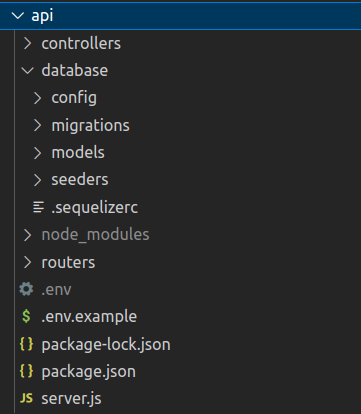
\includegraphics[scale=.50]{./Figures/api-estructura-archivos.png}
	\caption{Estructura de carpetas en patrón de desarrollo modular.}
	\label{fig:apiestructura}
\end{figure}

Dentro de cada una de las carpetas se encuentran los archivos Javascript correspondientes. El archivo \textit{server.js} es el punto de partida de la API y donde se realizan las configuraciones de conexión a bases de datos con Sequelize, configuración de Express, se definen los puertos a utilizar, la conexión MQTT, se declaran las rutas o \textit{routes}, entre otras configuraciones.

En el archivo \textit{package.json} se encuentran configuraciones y datos fundamentales para la aplicación, entre estas están: el nombre de la aplicación, la versión, descripción del proyecto, los scripts de inicio y ejecución, las dependencias del proyecto, bibliotecas y paquetes de terceros utilizados, las versiones específicas de las dependencias requeridas y la información de licencia. En este archivo se define, por ejemplo, el uso de Sequelize y Express y sus respectivas versiones.

El archivo .env es un archivo que no se versiona, esto significa que no se resguarda el historial de cambios del archivo, esto se debe a que contiene información sensible que debe mantenerse segura y no debe versionarse ni subirse a internet. En cada entorno dónde la aplicación sea instalada se deberá crear este archivo manualmente y escribir las definiciones de manera manual. Se declara, por ejemplo, usuario y contraseña para la conexión a base de datos, credenciales para conexión a \textit{broker} MQTT, direcciones IP o URL, conexión a Wi-Fi, entre otros datos sensibles.

En las siguientes secciones se detallan las carpetas \textit{routers} y \textit{controllers}.

\subsection{Ruteo de la API}
\label{subsec:apirouters}

En la carpeta \textit{routers} se encuentran los archivos Javascript que corresponden a las rutas que maneja Express para recibir las peticiones o \textit{requests} HTTP provenientes desde fuera de la API, generalmente desde el cliente \textit{frontend}.

En la figura \ref{fig:apiroutes} se muestran los archivos de ruteo que se crearon siguiendo el patrón modular, separando las rutas según su entidad o funcionalidad.

\begin{figure}[ht]
	\centering
	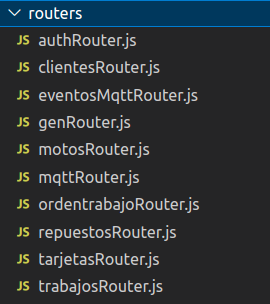
\includegraphics[scale=.50]{./Figures/api-routes.png}
	\caption{Estructura de archivos en carpeta de rutas.}
	\label{fig:apiroutes}
\end{figure}

En el archivo \textit{ordentrabajoRouter.js} se manejan las peticiones a rutas referentes a las órdenes de trabajo, de la misma manera para los demás archivos. 

A modo de ejemplo se presenta un fragmento de código de ruteo correspondientes a órdenes de trabajo:


\begin{lstlisting}[label=cod:routesot,caption=Código de ruteo para órdenes de trabajo.]
    /**
     * Nueva orden de trabajo
     * @params data, estado = espera
     * Recibe datos para la orden de trabajo
     * incluido el numero de tarjeta rfid
     */
    ordentrabajoRouter.post('/nueva',
        ordentrabajoCtrl.nuevaOrdenTrabajo);
\end{lstlisting}

En la declaración de esta ruta podemos observar que la dirección de la ruta en cuestión es \textit{/nueva} y se define con el método \textit{post()} en un objeto de router llamado \textit{ordentrabajoRouter}. Este método indica que la ruta es accesible mediante una solicitud HTTP POST, que es utilizada para enviar información a un servidor para crear un recurso.

Además, se especifica un controlador de ruta \textit{(handler)}. El controlador es una función que se ejecuta cuando se realiza una solicitud HTTP a la ruta especificada. En este caso, el controlador de ruta se llama \textit{nuevaOrdenTrabajo} y se define en el archivo \textit{ordentrabajoCtrl}, más adelante veremos en profundidad la carpeta \textit{controllers} y sus características.

Cuando se realiza una solicitud HTTP POST a la ruta \textit{/nueva}, Express ejecutará automáticamente la función \textit{nuevaOrdenTrabajo} definida en el controlador de ruta \textit{ordentrabajoCtrl}.

De esta manera se logra separar la lógica de ruteo de la lógica de procesos y acceso a datos, siguiendo el patrón modular mencionado previamente.

\subsection{Controladores de la API}
\label{subsec:apicontrollers}

Como se mencionó en la sección previa, los controladores son funciones que se ejecutan luego de resolver la ruta a la cual están asociados. 

En la figura \ref{fig:apicontrollers} se puede ver como en la carpeta \textit{controllers} se definieron los controladores siguiendo el patrón modular de desarrollo, teniendo en cuenta la entidad o la funcionalidad que se desea procesar.

\begin{figure}[ht]
	\centering
	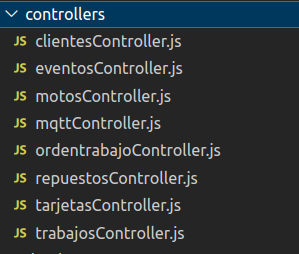
\includegraphics[scale=.50]{./Figures/api-controllers.png}
	\caption{Estructura de archivos en la carpeta \textit{controllers}.}
	\label{fig:apicontrollers}
	
\end{figure}

A modo de ejemplo se muestra a continuación un fragmento de código del controlador para obtener un listado de todas las motos de la base de datos:

\begin{lstlisting}[label=cod:routesot,caption=Código de controlador para obtener listado de motos.]
const {Moto} = require('../database/models/index');

const { Op, Sequelize } = require("sequelize");
const { response } = require('express');

//controller
const listarMoto = async (req, res)=>{
    try {
        const listadoMotos = await Moto.findAll({});
        
        return res.status(200).json({
            listadoMotos
        }); 

    } catch (error) {
        return res.status(400).json({
            error: error.message,
            message: 'Error listando motos'
        })
    }
    
};
\end{lstlisting}

La primera línea del código importa el modelo \textit{Moto} desde el archivo principal para los modelos de Sequelize \textit{index.js} ubicado en la carpeta \textit{models}. En la segunda línea, se importan las funciones \textit{Op y Sequelize} desde la librería Sequelize, estas funciones se utilizan para realizar operaciones y consultas en la base de datos. Luego, se define el controlador \textit{listarMoto} que se encarga de listar todas las motos de la base de datos. Dentro del controlador, se utiliza el método \textit{findAll()} de Sequelize para buscar todos los registros. Si la consulta a la base de datos se realiza con éxito, se devuelve un objeto \textit{JSON} con el listado de motos y un código de estado HTTP 200. En caso de que la consulta falle, se devuelve un objeto \textit{JSON} con el mensaje de error y un código de estado HTTP 400.

Finalmente, se exporta el controlador \textit{listarMoto} para que pueda ser utilizado en otras partes de la aplicación.

De manera similar se desarrollaron todos los controladores para las diferentes rutas de la aplicación. 

\subsection{Endpoints HTTP}
\label{subsec:apiendpointshttp}

Para la organización del desarrollo se realizó una tabla con todos los datos necesarios para los \textit{endpoints} o rutas de la API. 

En la figura \ref{fig:apiendpoints} se puede apreciar una parte de esta tabla correspondiente a las rutas para las órdenes de trabajo.

\begin{figure}[ht]
	\centering
	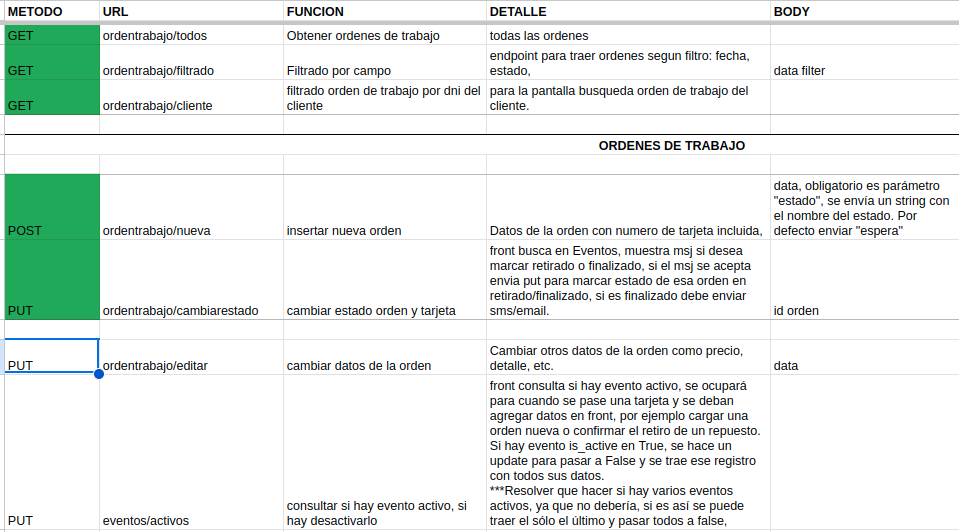
\includegraphics[scale=.40]{./Figures/api-endpoints.png}
	\caption{Tabla descriptiva de \textit{endpoints} o rutas de la API.}
	\label{fig:apiendpoints}
	
\end{figure}

A medida que se avanzó en el desarrollo se fueron marcando en verde las casillas de las rutas finalizadas, además se fue agregando más detalles o parámetros según requerimientos o necesidades.

\section{Comunicación MQTT}
\label{sec:mqttarquitectura}


\subsection{Diagrama MQTT}
\label{subsec:mqttdiagrama}

\begin{figure}[ht]
	\centering
	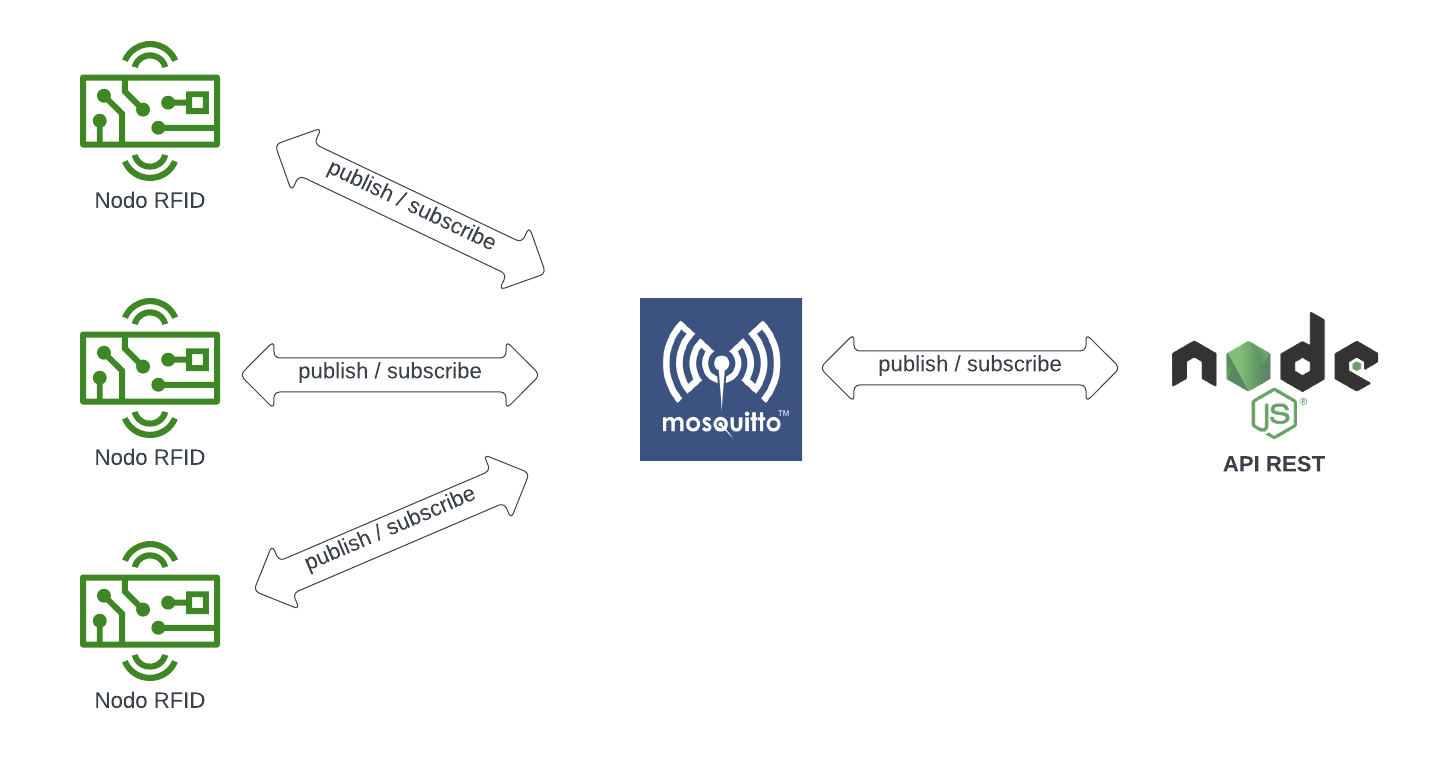
\includegraphics[scale=.15]{./Figures/mqtt-funciones.png}
	\caption{Diagrama de funciones MQTT.}
	\label{fig:mqttfunciones}
	
\end{figure}

En la figura \ref{fig:mqttfunciones} se pueden apreciar los distintos actores que intervienen en la comunicación MQTT del sistema. Los nodos RFID representan a cada ESP32 con el módulo lector RC522 mencionados en el capítulo \ref{subsec:esp32}, estos se encargan de marcar el estado específico de una órden de trabajo. En el centro se ubica el broker Mosquitto el cual se encarga de la distribución de los mensajes a los demás módulos y a la derecha está la API REST desarrollada en Node.js la cual recibe los mensajes provenientes de los nodos y realiza el proceso correspondiente, además de enviar publicaciones a modo de información y para \textit{logs}.

\subsection{Topics MQTT}
\label{subsec:mqtttopics}

Como se observa en la figura \ref{fig:mqtttopics}, se organizan los \textit{topics} MQTT en una tabla, en este caso, según el nodo o sensor y podemos ver en la cabecera de la tabla la información que representaremos para cada mensaje, el \textit{topic}, si es una publicación o suscripción, el mensaje en cuestión y una breve explicación de cuál es la función que cumple la comunicación.

\begin{figure}[H]
	\centering
	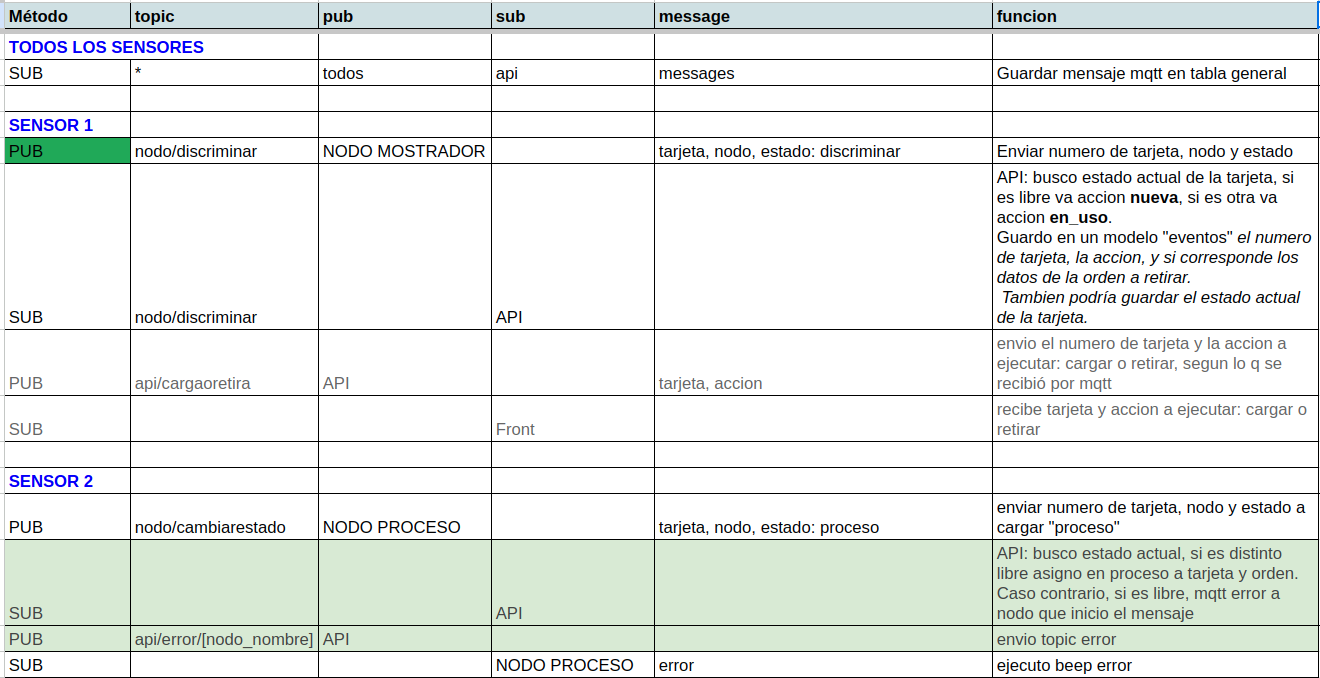
\includegraphics[scale=.30]{./Figures/mqtt-topics.png}
	\caption{Tabla de \textit{topics} MQTT.}
	\label{fig:mqtttopics}
\end{figure}

La lista completa de \textit{topics} implementados es la siguiente:
\begin{itemize}
\item *: API \textit{backend} se suscribe a todos los mensajes.
\item nodo/discriminar: emite nodo ``mostrador`` para ingresar o retirar órdenes de trabajo. Recibe API \textit{backend}.
\item nodo/cambiarestado: emite nodo ``proceso`` o ``finalizado`` para cambiar el estado de una órden de trabajo. Recibe API \textit{backend}.
\item api/error/mostrador: emite la API de \textit{backend} para informar un error en el proceso. Recibe nodo ``mostrador``.
\item api/error/proceso: emite la API de \textit{backend} para informar un error en el proceso. Recibe nodo ``proceso``.
\item api/error/finalizado: emite la API de \textit{backend} para informar un error en el proceso. Recibe nodo ``finalizado```.
\item api/confirmacion/mostrador: emite la API de \textit{backend} para informar proceso exitoso. Recibe nodo ``mostrador``.
\item api/confirmacion/proceso: emite la API de \textit{backend} para informar proceso exitoso. Recibe nodo ``proceso``.
\item api/confirmacion/finalizado: emite la API de \textit{backend} para informar proceso exitoso. Recibe nodo ``finalizado``.

\end{itemize}

\subsection{Broker MQTT}
\label{subsec:mqttbroker}

Para la implementación en el servidor del sistema en la Raspberry Pi del \textit{broker} MQTT ``Eclipse Mosquitto" se utilizó un servicio de Docker Compose el cual permite levantar el \textit{broker} y sus configuraciones.

En la figura \ref{fig:mqttestructuracarpetas} podemos observar la estructura de carpetas y archivos que se implementa en el contenedor de Docker para este servicio. 

\begin{figure}[H]
	\centering
	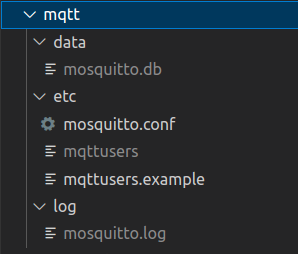
\includegraphics[scale=.60]{./Figures/mqtt-estructura-carpetas.png}
	\caption{Estructura de carpetas del servicio Eclipse Mosquitto en Docker.}
	\label{fig:mqttestructuracarpetas}
\end{figure}

\begin{itemize}
	\item En la carpeta \textit{data} se encuentra el archivo de base de datos \textit{mosquitto.db} donde se pueden persistir los mensajes MQTT según la configuración de persistencia implementada.
	\item En la carpeta \textit{etc} se encuentra el archivo de configuración principal del \textit{broker}: \textit{mosquitto.conf}, aquí se declaran todos los parámetros con los cuales Docker Compose levantará el servicio. El archivo \textit{mqttusers} persiste de manera encriptada las credenciales de acceso para los clientes MQTT, estos usuarios son administrados por línea de comando en la terminal \textit{bash} ingresando al contenedor específico. Por último se agregó un archivo con el ejemplo de comandos para administrar usuarios: \textit{mqttusers.example}.
	\item La carpeta \textit{log} contiene el archivo \textit{mosquitto.log} donde se registran todos los logs del servicio y que sirven para hacer un \textit{debug} o \textit{test} del mismo.	
\end{itemize}


\subsection{MQTT en nodos}
\label{subsec:mqttnodos}
Para implementar las comunicaciones MQTT en los nodos ESP32 se utilizó la biblioteca de código abierto PubSubClient \citep{WEBSITE:pubsubclient} la cual permite conexiones con servidores MQTT, publicar mensajes y suscribirse a los mensajes recibidos.

Como se describió en el capítulo \ref{Chapter1} Cada nodo representa uno o más estados específicos en la cadena de procesos que se realizan en la empresa. Estos estados son declarados en el código fuente del microcontrolador ESP32, específicamente en un archivo de entorno, de manera que pueda ser modificado fácilmente en caso de ser necesario.

A continuación se describen los nodos y sus estados utilizados:

\begin{itemize}
\item Nodo 1, ``mostrador``: este nodo cumple la función de comunicar a la API REST por medio de MQTT el número de tarjeta que ha sido leída en el mostrador de atención a clientes de la empresa. De esta manera la API REST se encargará de asignar los estados ``espera`` o ``retirado`` a las órdenes de trabajo según corresponda.

\item Nodo 2, ``proceso``: este nodo se encarga de comunicar a la API REST que debe cambiar el estado de la órden de trabajo a ``proceso``, la API REST reconoce que el mensaje proviene de este nodo por el ``topic`` por el cual se envía el mensaje, y consulta a la base de datos qué órden de trabajo tiene el número de tarjeta recibida para ejecutar la actualización.

\item Nodo 3, ``finalizado``: de la misma manera que en el nodo 2, en este sensor se informa a la API REST que debe cambiar el estado de la órden de trabajo asociada a la tarjeta leída a ``finalizado``.
\end{itemize}

De esta manera el ciclo de lecturas de los nodos para una órden de trabajo es el siguiente: 

\begin{enumerate}
\item Nodo ``mostrador``, se asigna el estado ``espera``.
\item Nodo ``proceso``, se asigna el estado ``proceso``.
\item Nodo ``finalizado``, se asigna el estado ``finalizado``.
\item Nodo ``mostrador``, se asigna el estado ``retirado``.
\end{enumerate}

Cuando un nodo envía o recibe una señal MQTT emite alertas sonoras para informar al usuario si la operación correspondiente tuvo éxito o fracaso. En la figura \ref{fig:mqttsonidosnodos} se puede observar cómo se implementaron estas señales sonoras en los nodos. Además podemos ver que existen dos opciones de sonidos, una es en forma de una sola nota denominada en la tabla \textit{Sonidos Clásicos} y otra es en forma de una melodía denominada \textit{Melodías}. Se configura en cada nodo la opción deseada desde las variables de entorno. Además se realiza en el código una validación para asegurarse que el tipo de \textit{buzzer} instalado es compatible con la opción \textit{Melodía}, en caso que no lo sea se ejecuta por defecto la opción \textit{Sonidos Clásicos}

\begin{figure}[H]
	\centering
	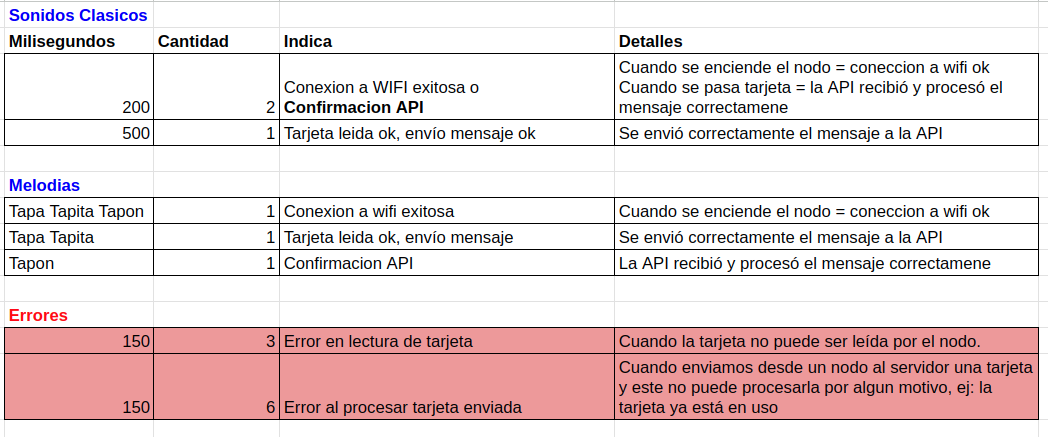
\includegraphics[scale=.40]{./Figures/mqtt-sonidos-nodos.png}
	\caption{Tabla de detalles de sonidos de nodos.}
	\label{fig:mqttsonidosnodos}
\end{figure}



\subsection{MQTT en API REST}
\label{subsec:mqttapi}

Se definió en la estructura de la API REST, descrita en el capítulo \ref{subsec:apipatron}, una sóla ruta de entrada en el archivo principal de configuración \textit{server.js}, dónde se realiza la conexión al \textit{broker} MQTT y se subscribe a todos los \textit{topics} utilizando para ello el símbolo \#. 

Configuración y conexión a \textit{broker} MQTT:
\begin{lstlisting}[label=cod:mqttapiconect,caption= Configuración y conexión a \textit{broker} MQTT en API REST.]
 // mqtt config
    const mqtt = require('mqtt')
    const host = process.env.MQTT_SERVER
    const port = process.env.MQTT_PORT
    const clientId = `api_mqtt_${Math.random().toString(16).slice(3)}`
    
    // mqtt connect function
    const connectUrl = `mqtt://${host}:${port}`
    const mqtt_client = mqtt.connect(connectUrl, {
      clientId,
      clean: true,
      connectTimeout: 4000,
      username: process.env.MQTT_USER,
      password: process.env.MQTT_PASSWORD,
      reconnectPeriod: 3000,
    })
\end{lstlisting}

Como se puede observar en el código \ref{cod:mqttapiconect} se traen la mayoría de los parámetros desde las variables de entorno, esto se realiza para mantener un código limpio y que sea fácil de mantener, en caso de requerir algún cambio se realiza directamente en el archivo de variables de entorno evitando tener que cambiar en varias partes del código.

Primero se importa la librería MQTT y se definen las variables correspondientes al \textit{host} y puerto del \textit{broker}, así como un \textit{clientId} generado aleatoriamente. Luego se define la función de conexión al \textit{broker}, utilizando la URL compuesta por el \textit{host} y \textit{puerto} definidos anteriormente, y se especifican las opciones de conexión, incluyendo el \textit{clientId} generado, la limpieza de sesión en la conexión, un tiempo de espera de conexión de 4 segundos, el nombre de usuario y contraseña para la conexión, y un período de reconexión de 3 segundos.


Subscripción a todos los \textit{topics}:

\begin{lstlisting}[label=cod:mqttapisub,caption=Subscripción a \textit{topics} en API REST.]
// subscribe to topics
    const topic = process.env.MQTT_TOPIC_ALL;
    mqtt_client.on('connect', () => {
      console.log('mqtt client Connected')
      mqtt_client.subscribe([topic], () => {
        console.log(`API Subscribe to topic '${topic}'`)
      })
    })
\end{lstlisting}

En el código \ref{cod:mqttapisub}, en la línea 2 se trae desde las variables de entorno el \textit{topic} correspondiente. Luego se inicia la conexión con el método \textit{on} y se realiza la suscripción con el método \textit{subscribe}. 

Luego los mensajes se rutean a un controlador MQTT que procesa todos los mensajes y siguiendo un flujo condicional realiza las acciones correspondientes.

A continuación se presenta un diagrama del flujo del código fuente para resolver los procesos según el mensaje MQTT recibido:

\begin{figure}[H]
	\centering
	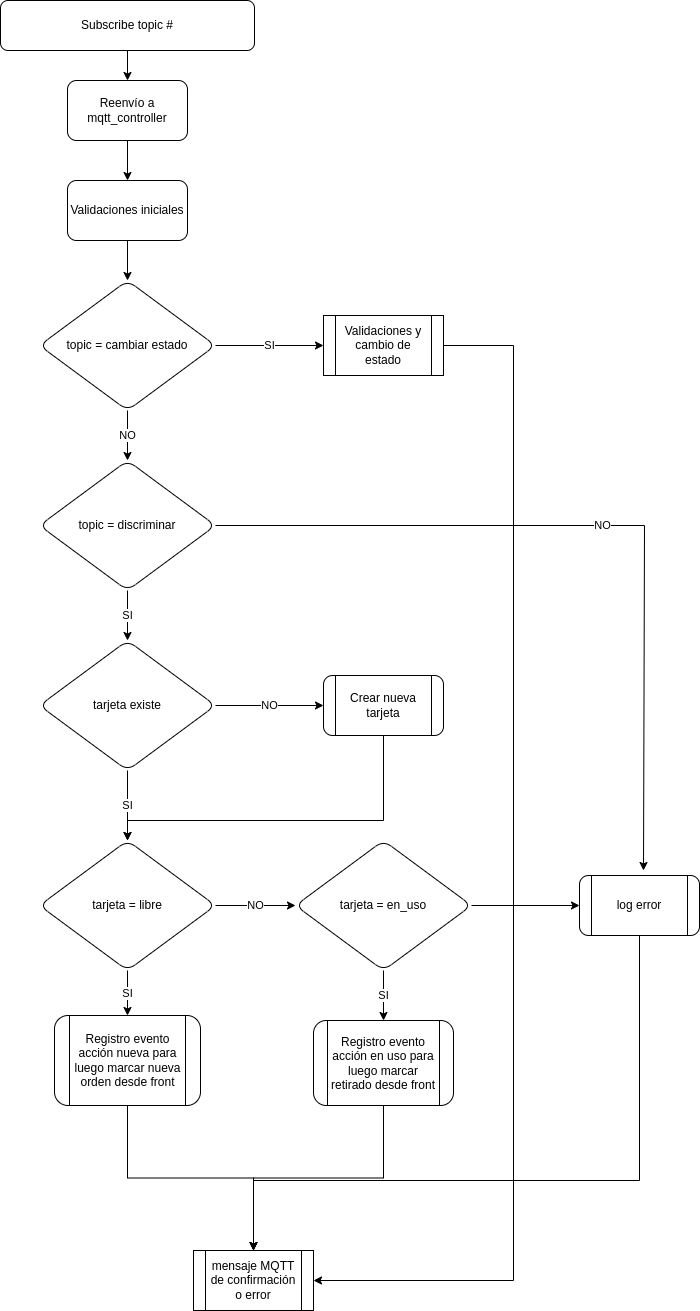
\includegraphics[scale=.50]{./Figures/mqtt-controller-api.png}
	\caption{Flujo de código fuente para MQTT en API REST.}
	\label{fig:mqttcontrollerapi}
\end{figure}

Como puede observarse en la figura \ref{fig:mqttcontrollerapi} las validaciones dependen tanto del \textit{topic} recibido como del estado de la tarjeta. De acuerdo a eso se realizan los procesos correspondientes y se devuelve siempre un mensaje MQTT al nodo emisor el cual, de acuerdo al mensaje recibido, emitirá una señal sonora a través del \textit{buzzer} para informar al usuario si la acción tuvo éxito o no.


\section{API para mensajería}
\label{sec:apimessenger}

Para el envío de mensajes por la aplicación \textit{WhatsApp} \cite{whatsapp} se utilizó una API adicional \cite{api-whatsapp-ts} la cual fue personalizada para las necesidades de este sistema.

En esta sección se detalla cómo se implementó una API de mensajería para \textit{WhatsApp}.

Esta API permite al usuario de la aplicación conectarse a \textit{WhatsApp} con su teléfono móvil y enviar mensajes desde la aplicación a los clientes de manera automática.

\subsection{Implementación}
\label{subsec:apimessengerimplementación}

Para implementar está API se creó un contenedor en Docker de manera tal de separar este servicio del resto de los demás siguiendo una arquitectura de tipo microservicios \cite{microservices-docs}.

El patrón de desarrollo es similar al de la API REST detallada en el capítulo \ref{sec:arquitecturaapirest} y también está desarrollada en Node.js y Express, por lo que su personalización fue sencilla para este trabajo.

Se modificó el código fuente de la API para poder autenticarse desde el frontend al servicio de \textit{WhatsApp}, permitiendo que desde el frontend se pueda realizar una petición por medio del protocolo HTTP y que la API devuelva un código QR \cite{qr-code} en formato SVG \cite{svg-format} para que el usuario pueda realizar la conexión. 

En el ruteo del proyecto se añadió un endpoint para obtener un código QR de autenticación:

\begin{lstlisting}[label=cod:apimessengerroute,caption=Endpoint para obtener código QR.]
router.get("/", leadCtrl.getQrCode);
router.get("/regenerateqr", leadCtrl.regenerateQrCode);
\end{lstlisting}

Luego en el controlador se realiza la lógica correspondiente:

\begin{lstlisting}[label=cod:apimessengercontroller,caption=Controlador de ruta para obtener código QR.]
  public getQrCode = async(req: Request,res: Response)=>{
    const path = `${process.cwd()}/tmp`;
    res.setHeader('Content-Type', 'image/svg+xml');
    res.sendFile(`${path}/qr.svg`);
  }

  public regenerateQrCode = async(req: Request,res: Response)=>{
    console.log("logout test");
    const response = await this.leadCreator.logoutSrv();
    res.send(response);
  }
\end{lstlisting}

La primera función, llamada \textit{getQrCode}, es un controlador que se encarga de mostrar el código QR para autenticar la sesión de \textit{WhatsApp} en la aplicación. Para hacerlo, el código utiliza la función \textit{res.sendFile()} para enviar el archivo \textit{qr.svg} que se encuentra en la carpeta \textit{tmp} del directorio actual del proyecto. Además, se establece el encabezado de respuesta \textit{Content-Type} a \textit{image/svg+xml} para indicar que se está enviando un archivo SVG.

La segunda función, llamada \textit{regenerateQrCode}, es otro controlador que se encarga de cerrar la sesión de \textit{WhatsApp} actual y volver a generar un nuevo código QR. Para hacerlo, se llama a una función \textit{logoutSrv()} que se encuentra en la clase \textit{leadCreator}. Luego, se envía la respuesta al cliente con la respuesta recibida de la función \textit{logoutSrv()}.


\section{Desarrollo frontend}
\label{sec:secarquitecturafrontend}
Para el desarrollo de las interfaces de usuario se utilizó el framework Ionic \cite{WEBSITE:ionic}, implementando de esta manera el lenguaje Javascript tanto en el \textit{backend} como en el \textit{frontend}.

\subsection{Patrón de desarrollo}
\label{subsec:frontpatron}

Se implementó el patrón de diseño MVC \citep{mvc} \textit{(Modelo-Vista-Controlador)} para estructurar las aplicaciones web. Este patrón divide la aplicación en tres capas principales: el modelo, el cual representa los datos y la lógica de negocio, la vista, que representa las interfaces de usuario, y el controlador, que actúa como intermediario entre la vista y el modelo.

También se utilizaron otros patrones de diseño, como el patrón de ``Inyección de Dependencias`` \citep{dependency-injection} \textit{Dependency Injection Pattern} y el patrón de ``Observador`` \citep{observer-pattern} \textit{Observer Pattern}. Estos patrones son utilizados para mejorar la escalabilidad, la flexibilidad y la mantenibilidad de las aplicaciones desarrolladas con Ionic.

En la capa de la vista se utilizaron las páginas, componentes y módulos de Ionic. Las páginas son plantillas en HTML o lenguaje IONIC. Los componentes son elementos visuales que se desarrollan en lenguajes HTML, CSS y Javascript y son implementados en las páginas. Los módulos son grupos de páginas y componentes. 

En la capa de controlador se utilizó un archivo Javascript con las funciones y la lógica para cada componente, dándole funcionalidad al mismo. 

En la capa de modelo se implementaron los servicios de Ionic, estos son clases que contienen métodos y lógica de negocio para recuperar datos de la API. 

Además se utilizó el manejo de rutas para mapear las URL a las páginas. Se asignó a cada módulo un archivo de rutas independiente para el manejo fluido de las páginas.

En la figura \ref{fig:frontmvc} podemos observar una representación del flujo utilizando este patrón. 

\begin{figure}[H]
	\centering
	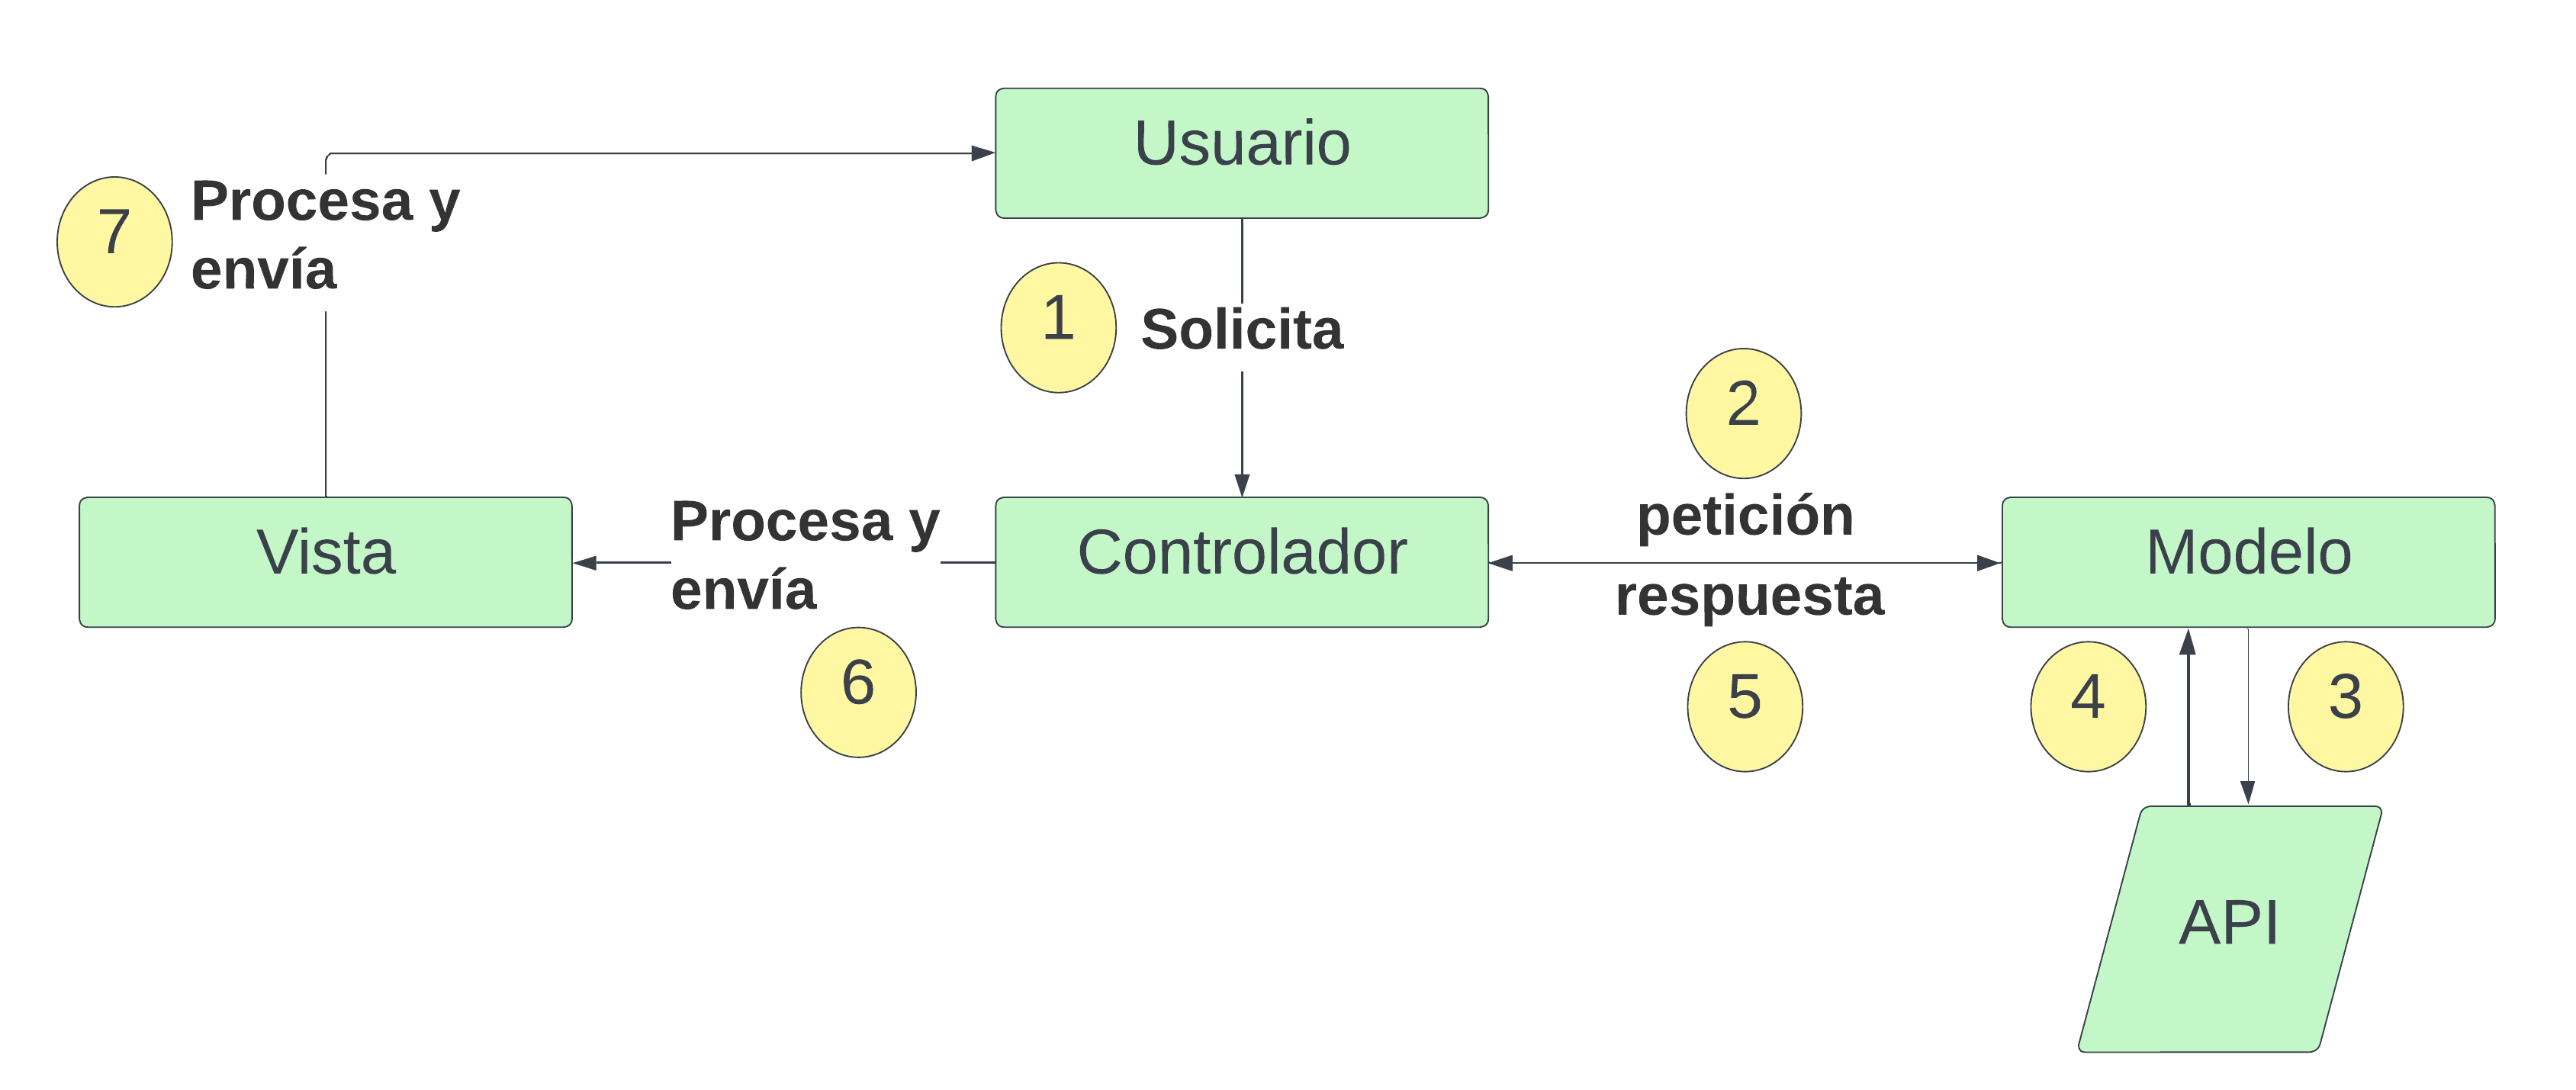
\includegraphics[scale=.15]{./Figures/front-mvc.png}
	\caption{Flujo en MVC.}
	\label{fig:frontmvc}
\end{figure}

Por ejemplo, para el desarrollo del módulo de listar órdenes de trabajo implementando este patrón, el flujo sería el siguiente:

\begin{enumerate}
\item Usuario solicita a través de su navegador la URL \textit{ordenestrabajo/listar}.
\item El \textit{routing} mapea la URL al controlador \textit{listar.page.ts} que se encuentra en el módulo \textit{listar.module.ts}. El controlador llama al servicio \textit{ordentrabajo.services.ts}.
\item El servicio hace una petición HTTP por medio del método GET a una ruta de la API de \textit{backend}. 
\item La API responde con los datos de la lista en formato JSON.
\item El servicio entrega esos datos al controlador en formato JSON.
\item El controlador procesa los datos, realiza validaciones y filtros necesarios, ordena los datos, etc.
\item La vista procesa los datos, los inserta en una tabla, aplica los diseños CSS, etc. Luego envía la vista con los datos al usuario quien la visualizará en su navegador. 
\end{enumerate}

De esta manera se implementó este patrón de desarrollo para todos los componentes y módulos del \textit{frontend}.

\subsection{Interfaces de usuario}
\label{subsec:frontinterfaces}

Teniendo en cuenta el flujo general del sistema presentado en el capítulo \ref{sec:flujogeneral} y los requerimientos para un sistema que sea amigable con el usuario y de diseño adaptable a diferentes dispositivos, se desarrollaron las interfaces de usuario utilizando los componentes nativos de Ionic para diseño de interfaces junto a CSS para personalizar estilos y javascript para funcionalidades. 

Las interfaces de usuario que se desarrollaron fueron:

\begin{enumerate}
\item Nueva: para añadir una nueva órden de trabajo.
\item Listar: para listar todas las órdenes de trabajo.
\item Retirar: para retirar una órden de trabajo.
\item Clientes: de tipo modal, para añadir o buscar un cliente.
\item Motos: de tipo modal, para añadir o buscar una motocicleta.
\item QR: para mostrar el código QR para autenticación en \textit{Whatsapp}.
\end{enumerate}

\subsubsection{Nueva órden de trabajo}
\label{subsubsec:frontnuevaorden}
En la figura \ref{fig:nuevafull1} podemos observar los primeros campos del formulario a rellenar para cargar una nueva órden de trabajo.

\begin{figure}[H]
	\centering
	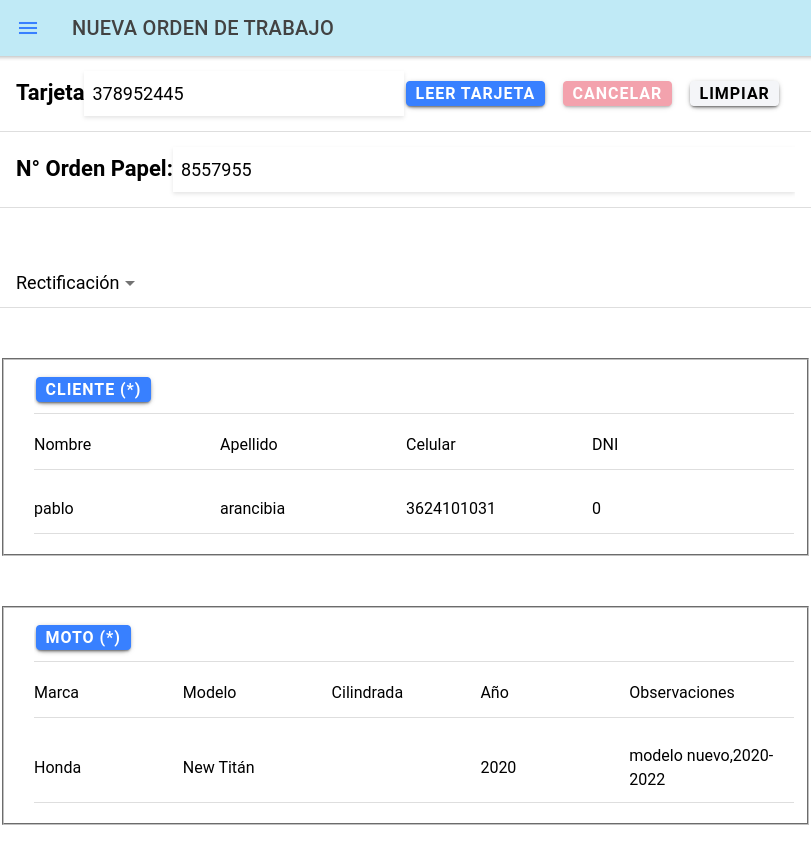
\includegraphics[scale=.30]{./Figures/nueva-full-1.png}
	\caption{Interfaz de usuario para nueva órden de trabajo.}
	\label{fig:nuevafull1}
\end{figure}


El usuario deberá hacer clic en el botón ``LEER TARJETA`` y luego pasar la tarjeta RFID por el lector ``mostrador``. De esta manera el sistema trae el número de tarjeta que fue seleccionada para asignar a la órden. Luego deberá cargar, si existe, un número de órden de manera manual el cual corresponde a un \textit{ticket} que usa actualmente la empresa.

Para cargar el tipo de trabajo, datos del cliente y la motocicleta se utilizan interfaces de tipo modal, las cuales se presentan a continuación:

En la figura \ref{fig:nuevatrabajo} se presenta la interfaz de tipo modal para seleccionar el tipo de trabajo a asignar a la órden.

\begin{figure}[H]
	\centering
	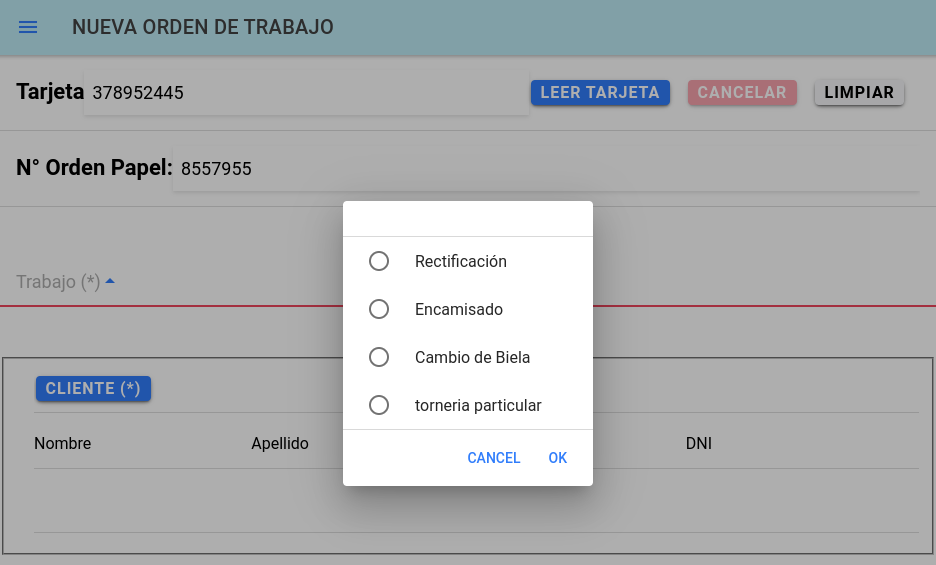
\includegraphics[scale=.30]{./Figures/nueva-trabajo.png}
	\caption{Interfaz de usuario de tipo modal para seleccionar tipo de trabajo.}
	\label{fig:nuevatrabajo}
\end{figure}

Para cargar o buscar los datos de clientes se utilizó el mismo componente, reutilizando así parte del código fuente. Como podemos ver en las figuras \ref{fig:nuevacliente1} y \ref{fig:nuevacliente2}, también se usa el tipo de interfaz modal.

\begin{figure}[H]
	\centering
	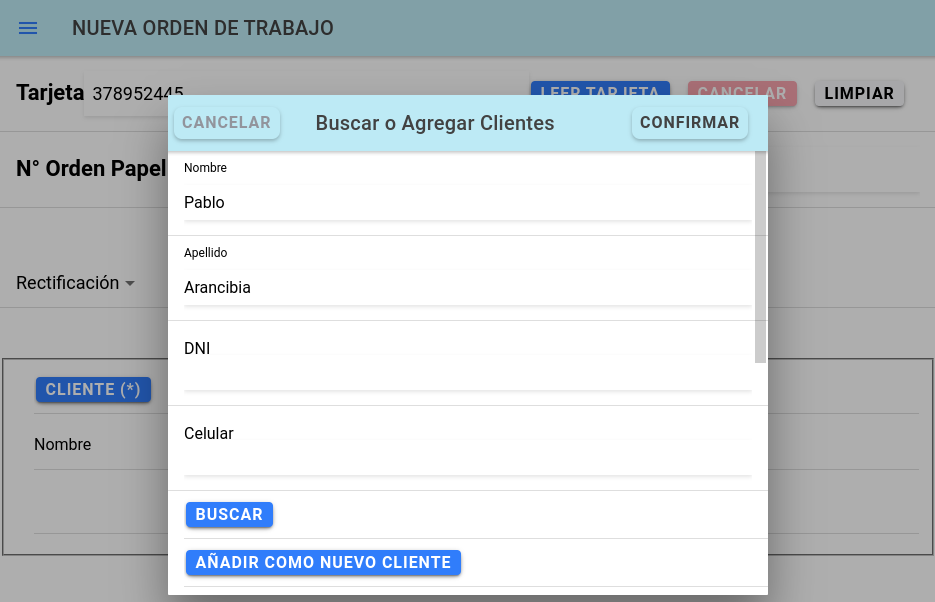
\includegraphics[scale=.30]{./Figures/nueva-clientes-1.png}
	\caption{Interfaz de usuario de tipo modal para seleccionar o buscar cliente.}
	\label{fig:nuevacliente1}
\end{figure}

En la figura \ref{fig:nuevacliente2} podemos observar el resultado de una búsqueda de clientes. Se selecciona el que se desea asignar y se hace clic en ``CONFIRMAR``.

\begin{figure}[H]
	\centering
	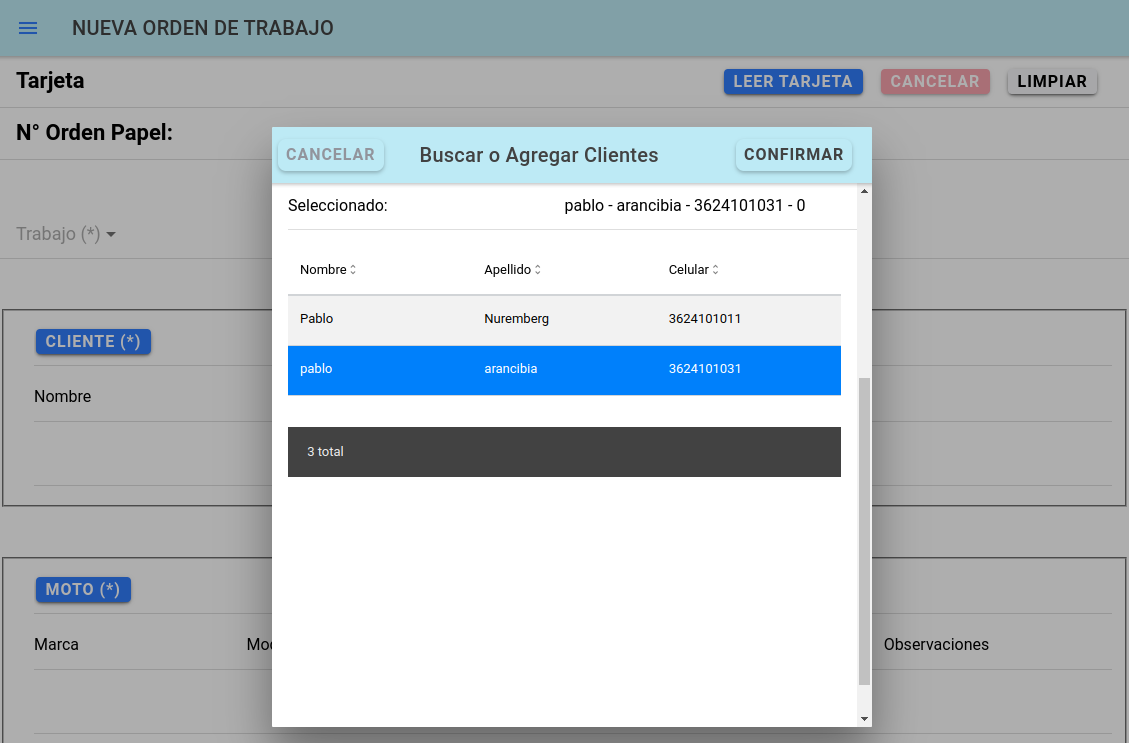
\includegraphics[scale=.30]{./Figures/nueva-clientes-2.png}
	\caption{Interfaz de usuario de tipo modal con el resultado de búsqueda de clientes.}
	\label{fig:nuevacliente2}
\end{figure}

De la misma manera se puede seleccionar o crear un registro de datos de una nueva motocicleta para asignar a la órden. En las figuras \ref{fig:nuevamoto1} y \ref{fig:nuevamoto2} vemos las interfaces modales.


\begin{figure}[H]
	\centering
	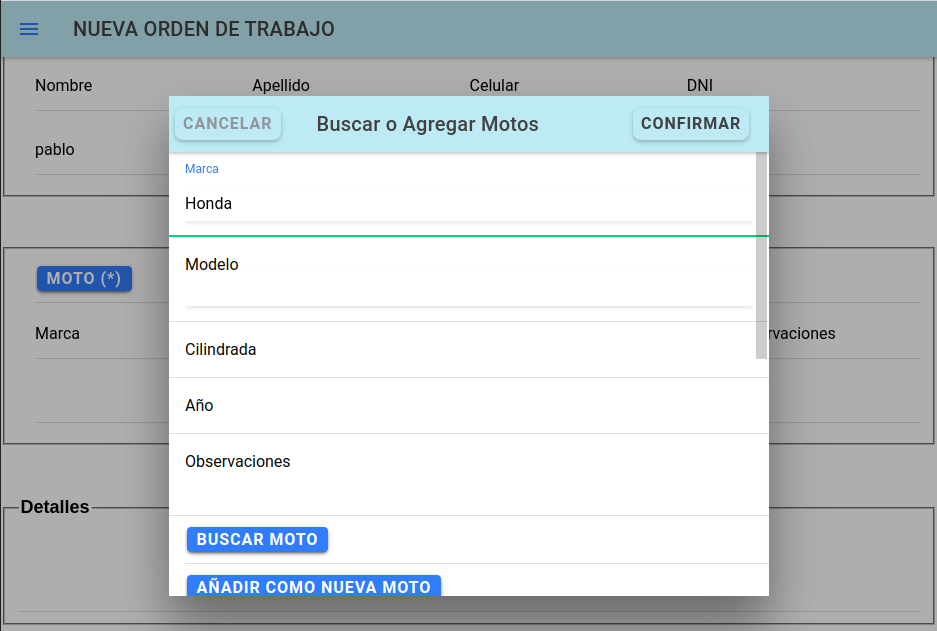
\includegraphics[scale=.30]{./Figures/nueva-moto-1.png}
	\caption{Interfaz de usuario de tipo modal para seleccionar o buscar motocicleta.}
	\label{fig:nuevamoto1}
\end{figure}

\begin{figure}[H]
	\centering
	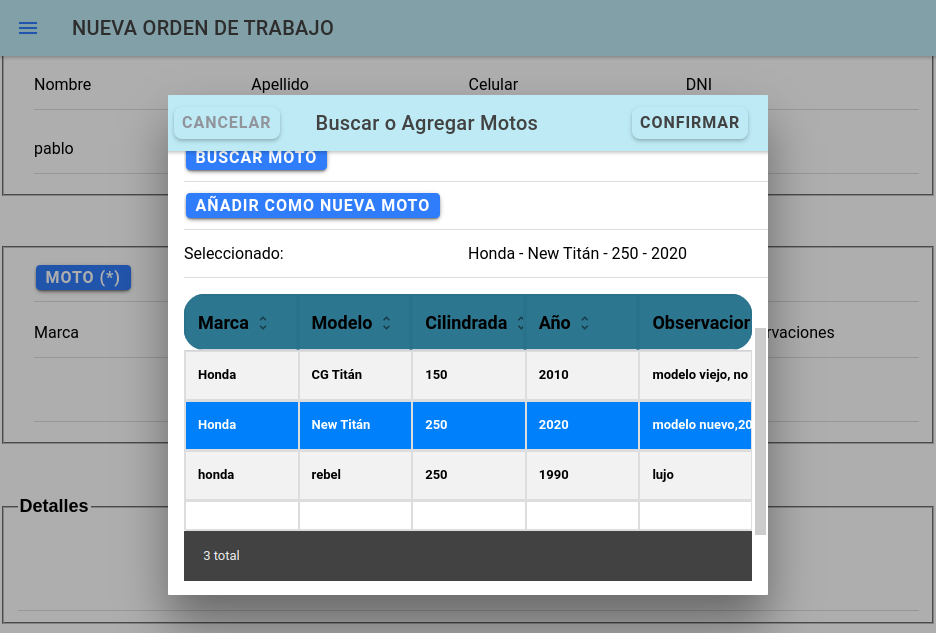
\includegraphics[scale=.30]{./Figures/nueva-moto-2.png}
	\caption{Interfaz de usuario de tipo modal con el resultado de búsqueda de motocicletas.}
	\label{fig:nuevamoto2}
\end{figure}

Volviendo a la segunda sección del formulario para agregar una nueva órden, ya habiendo cargado el número de tarjeta, el tipo de trabajo, el cliente y la motocicleta, continuamos con los campos que se representan en la figura \ref{fig:nuevafull2}.

 
\begin{figure}[H]
	\centering
	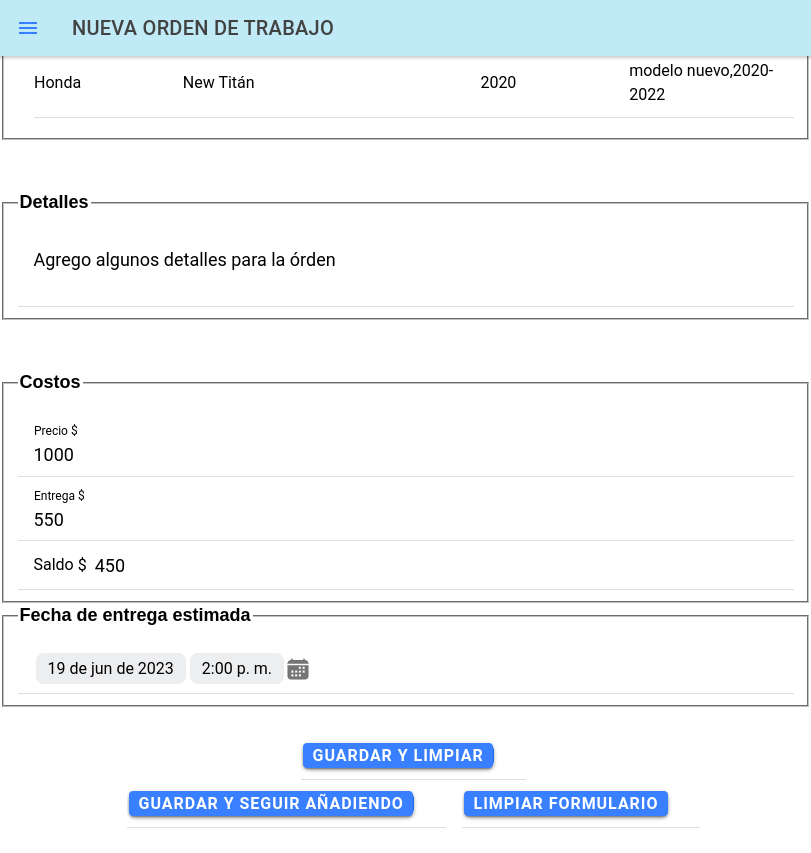
\includegraphics[scale=.30]{./Figures/nueva-full-2.png}
	\caption{Interfaz de usuario para nueva órden de trabajo.}
	\label{fig:nuevafull2}
\end{figure}

En esta sección podemos agregar detalles, costos y fecha de entrega estimada.

\begin{itemize}
\item Detalles: para agregar algunas observaciones a la órden en formato de texto
Costos: están separados en 3 campos: el precio total de la órden, la entrega que realiza el cliente cuando deja el repuesto y el saldo restante. 
\item Fecha de entrega estimada: al seleccionar la fecha saldrá un calendario de tipo modal para seleccionar el día y la hora de entrega. 
\end{itemize}


Por último sólo queda guardar la órden, para ello se pueden realizar dos acciones: 

\begin{itemize}
\item GUARDAR Y LIMPIAR: esta opción se utilizará cuando el cliente sólo deje un repuesto para trabajar de manera tal que se guarda el registro y se limpia completamente el formulario

\item GUARDAR Y SEGUIR AÑADIENDO: cuando el mismo cliente tiene varios repuestos para dejar, de esta manera se guarda el registro pero se mantienen los datos del cliente en el formulario. 
\end{itemize}

La última opción corresponde a ``LIMPIAR FORMULARIO`` que borra los datos del formulario sin guardar ningún registro.


\subsubsection{Listar órdenes de trabajo}
\label{subsubsec:frontlistarordenes}

En la figura \ref{fig:listado1} podemos observar la interfaz gráfica para donde se listan las órdenes de trabajo según las opciones seleccionadas.

\begin{figure}[H]
	\centering
	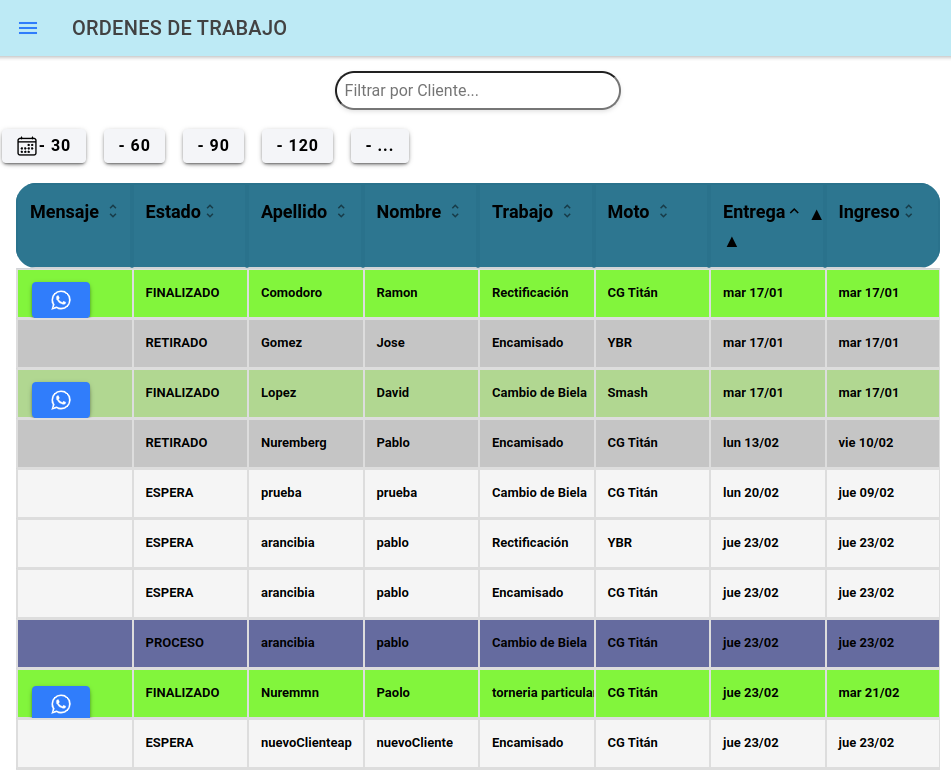
\includegraphics[scale=.30]{./Figures/listado-1.png}
	\caption{Interfaz de usuario para listar las órdenes de trabajo.}
	\label{fig:listado1}
\end{figure}

Las opciones en esta interfaz son:

\begin{itemize}
\item Filtrado: se puede filtrar por cualquier campo de la tabla, una vez que se filtran los resultados, la información se sigue actualizando en tiempo real, por lo que si una fila cambia de estado, se verá de todas maneras el cambio.

\item Rango de días: en la parte superior de la tabla se pueden observar 5 botones, estos representan al rango de días hacia atrás que se desea mostrar los registros. Además la tabla muestra al usuario una paginación navegable en la parte inferior si los registros son mayores a 25. El último botón de este grupo corresponde a mostrar el historial completo de registros.

\item Ordenamiento por campos: al hacer clic en la cabecera de la tabla se puede ordenar los elementos de manera múltiple, por ejemplo en primer órden la fecha de entrega y en segundo órden el apellido del cliente, así sucesivamente en múltiples campos.

\item Órden de columnas: se pueden ordenar los campos haciendo clic y arrastrando el campo deseado al órden correspondiente. Por ejemplo se puede arrastrar el campo ``Estado`` en la primera columna.
\end{itemize}

Para una mejor visualización de los estados de los trabajos se asignó un color específico para cada estado, de esta manera es más fácil identificar rápidamente el estado de los trabajos. Se utilizó la siguiente paleta de colores para los estados:

\begin{itemize}
\item Espera: color verde.
\item Proceso: color púrpura.
\item Finalizado: color verde brillante o verde opaco.
\item Retirado: color gris. 
\end{itemize} 

Además se asigna un botón en la columna ``Mensaje``, solamente a las filas de los trabajos que están en estado ``FINALIZADO``. Este botón tiene el logo de la aplicación \textit{WhatsApp} y se utiliza para enviar un mensaje al cliente informando que su trabajo está finalizado y listo para retirarse. En caso que el cliente todavía no fue alertado el color de la fila será verde brillante, si el cliente ya fue avisado el color de la fila será verde opaco. El usuario puede reenviar un mensaje a un cliente si lo desea sólo que el sistema lo alertará previamente.

En las figuras \ref{fig:listado2} y \ref{fig:listado3} vemos los alertas de tipo modal que se utilizan para confirmar cuando el usuario va a enviar o reenviar un mensaje a un cliente.

\begin{figure}[H]
	\centering
	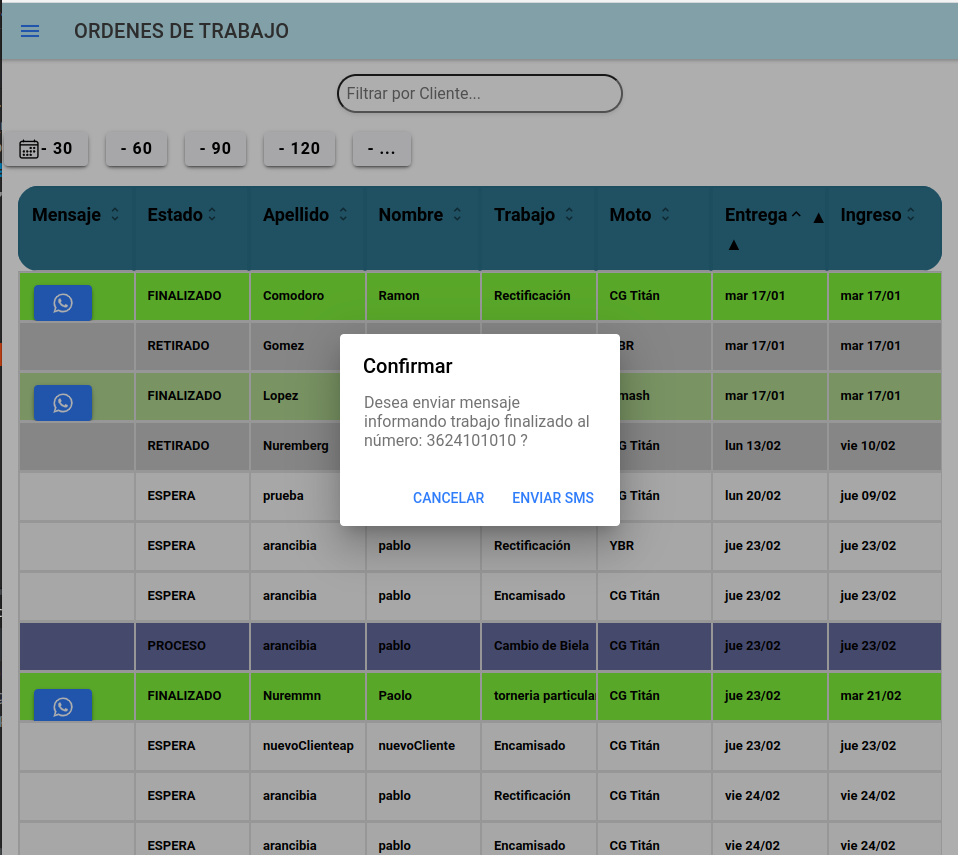
\includegraphics[scale=.30]{./Figures/listado-2.png}
	\caption{Confirmar envío de mensaje de texto al cliente.}
	\label{fig:listado2}
\end{figure}

\begin{figure}[H]
	\centering
	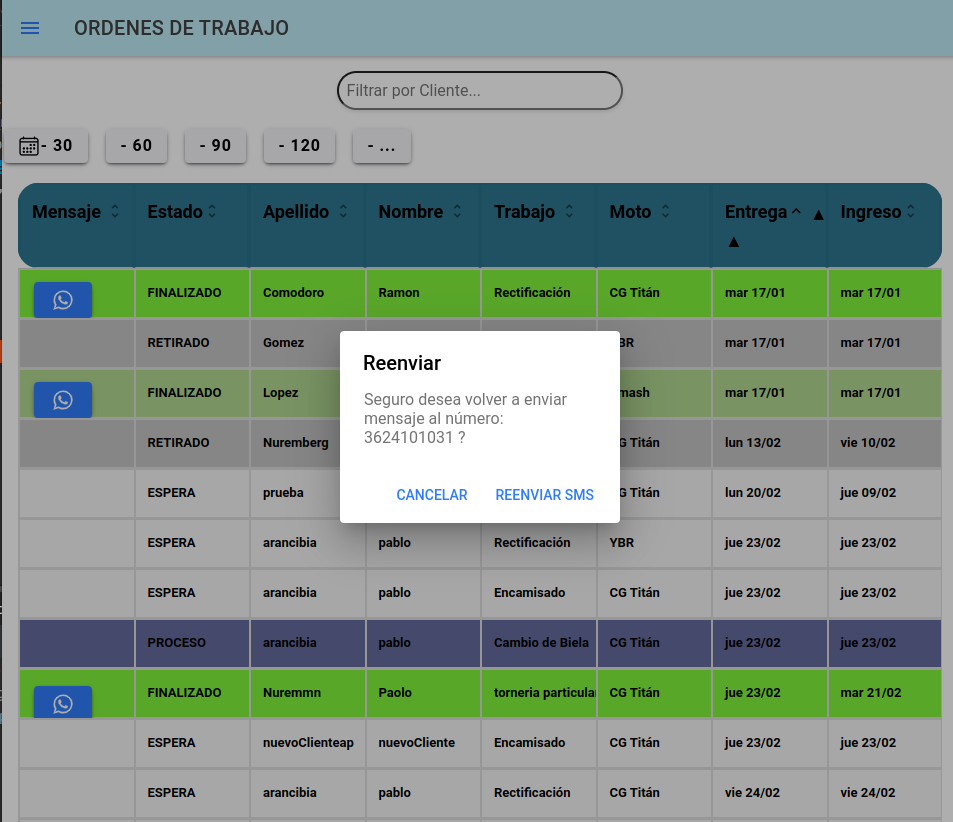
\includegraphics[scale=.30]{./Figures/listado-3.png}
	\caption{Confirmar reenvío de mensaje de texto al cliente.}
	\label{fig:listado3}
\end{figure}

Como se detalló en el capítulo \ref{sec:apimessenger} el mensaje llegá al cliente en su aplicación \textit{WhatsApp} como si fuera enviado desde el teléfono móvil del usuario, por lo que mostrará su número o el nombre por el cual el cliente lo tenga agendado, ya que la API de mensajería utiliza los servicios de \textit{WhatsApp} para hacer el envío y el usuario debe autenticarse previamente con su teléfono móvil y el código QR para utilizar el servicio.

\subsubsection{Retirar órden de trabajo}
\label{subsubsec:frontretirar}

Para retirar una órden se utiliza una metodología similar a la de agregar una nueva órden de trabajo. El usuario va hacer clic en un botón para activar la búsqueda de un evento, este evento será pasar la tarjeta RFID del repuesto por el nodo mostrador, una vez hecho esto el número de la tarjeta con todos los datos de la órden se cargará en la pantalla. 

El usuario puede modificar el precio de la órden en este punto y se actualizarán los datos de saldo. También puede agregar detalles para el retiro de la órden que quedarán registrados en la base de datos.

Una vez confirmado el retiro se guardan los registros y estados correspondientes y se asigna el estado ``libre`` a la tarjeta para que pueda ser reutilizada para una futura órden de trabajo.

De esta manera finaliza el ciclo de un repuesto que ingresa a la empresa, es procesado y retirado luego por el cliente.

En las figuras \ref{fig:retirar1} y \ref{fig:retirar2} vemos la interfaz para retirar una órden de trabajo.

\begin{figure}[H]
	\centering
	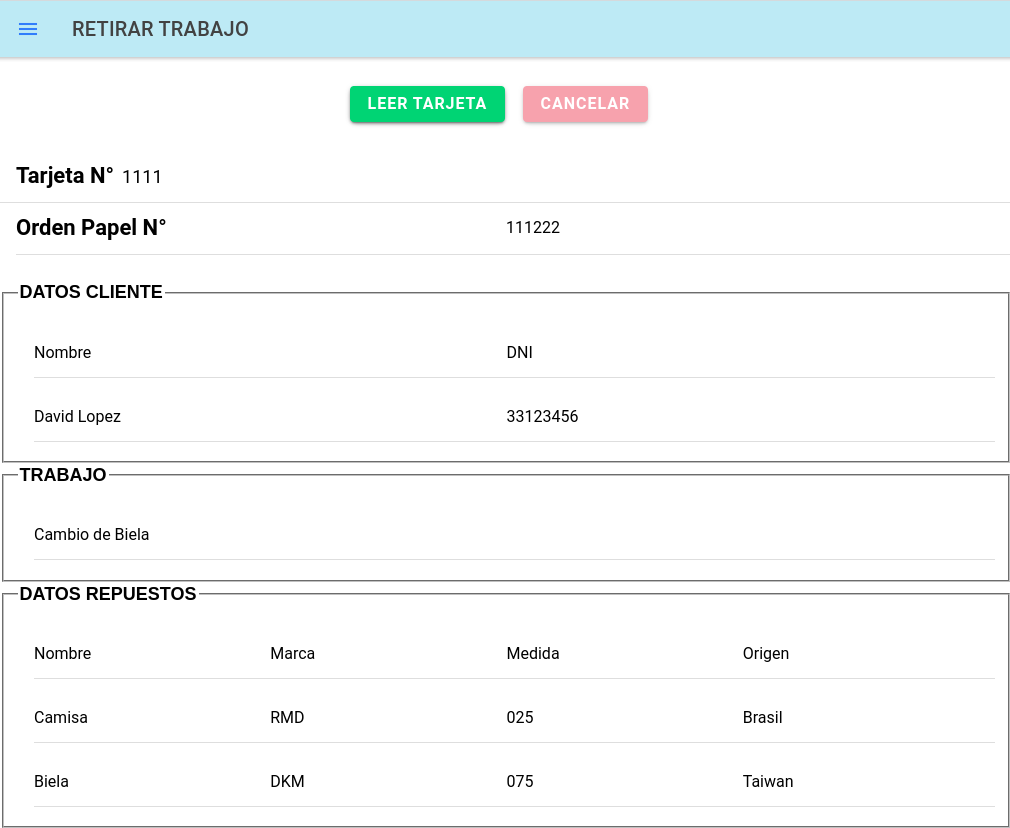
\includegraphics[scale=.30]{./Figures/retirar-1.png}
	\caption{Formulario para retirar órden de trabajo.}
	\label{fig:retirar1}
\end{figure}

\begin{figure}[H]
	\centering
	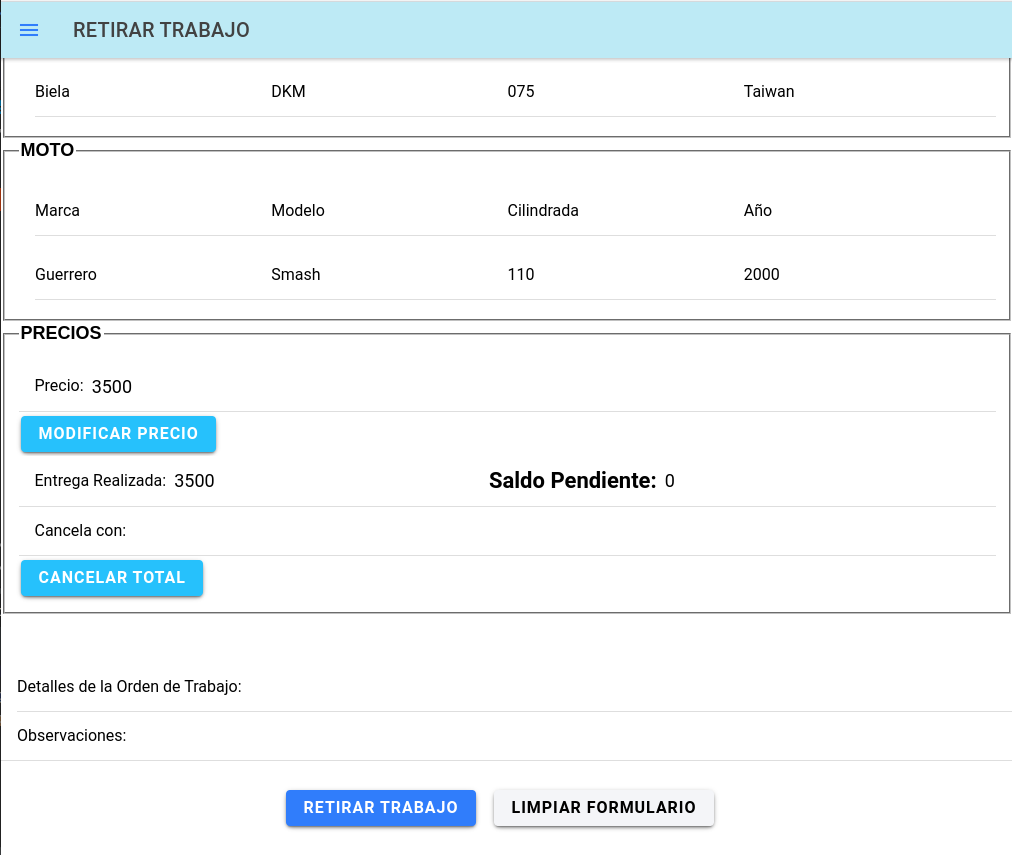
\includegraphics[scale=.30]{./Figures/retirar-2.png}
	\caption{Confirmar retiro de órden de trabajo.}
	\label{fig:retirar2}
\end{figure}

\subsubsection{Autenticación a API de mensajería}
\label{subsubsec:frontqr}

Para la autenticación a la API de mensajería se utiliza un código QR que se obtiene consultando dicha API por protocolo HTTP. La misma devuelve un archivo SVG que se muestra en la interfaz gráfica del usuario para que pueda ser escaneada por su teléfono móvil y de esta manera acceder a las funciones de envío de mensajes a clientes.

En la figura \ref{fig:frontqr} podemos ver la interfaz para autenticarse mediante código QR. También se puede observar el botón ``ACTUALIZAR`` para refrescar el código por uno nuevo´.

\begin{figure}[H]
	\centering
	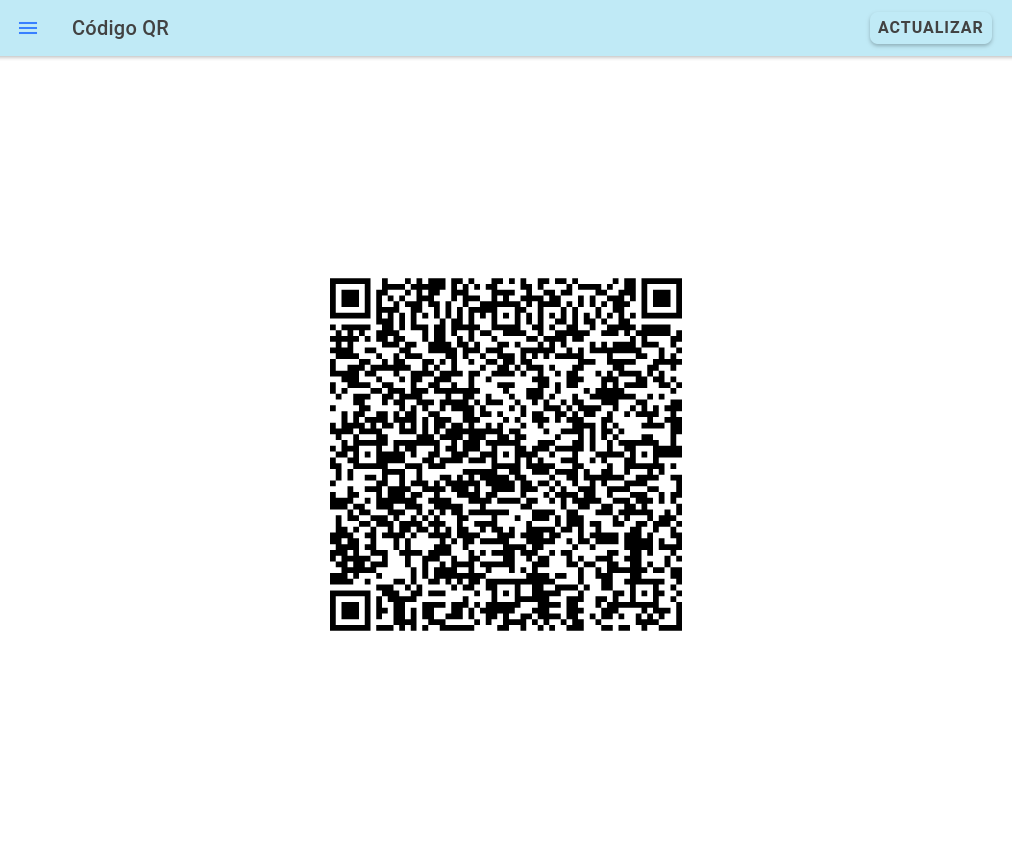
\includegraphics[scale=.30]{./Figures/qr-page.png}
	\caption{Interfaz para autenticación en API de mensajería.}
	\label{fig:frontqr}
\end{figure}

\section{Arquitectura de servidor}
\label{sec:server}

Para el despliegue de los servicios desarrollados se implementó una arquitectura de contenedores utilizando Docker y Docker Compose en una Raspberry Pi 4.

Para cada proyecto se creó un archivo Dockerfile para el manejo del contenedor correspondiente, a su vez se centraliza el despliegue de estos contenedores en un archivo \textit{yml} de Docker Compose, donde también se levantan servicios directamente sin utilizar un Dockerfile particular. 

En esta sección se detalla la implementación de contenedores y servicios en el servidor.

\subsection{Implementación de contenedores}
\label{subsec:contenedores}

A continuación se representa el código fuente utilizado en Docker Compose para el despliegue de todos los contenedores de cada proyecto o servicio utilizado:

\begin{lstlisting}[label=cod:dockercompose,caption=Código de Docker Compose.]
version: '3'

services:
    db:
        container_name: mysqldb
        restart: always
        image: mysql
        env_file:
        - .env_mysql/.mysql.env
        volumes:
            - ./sql-data/db:/var/lib/mysql
        ports: 
            - "3306:3306"
    api:
         depends_on: 
             - db 
         container_name: backendapi
         restart: always
         build:
             context: .
             dockerfile: Dockerfile
         command: bash -c 'while !</dev/tcp/db/3306; do sleep 1; done; npm run dev'
         ports:
             - "3001:3001"
         env_file:
         - ./api/.env
         volumes:
             - ./:/app
    mosquitto:
        image: eclipse-mosquitto
        container_name: mosquittobroker
        ports:
            - "1883:1883"
            - "9001:9001"
        volumes:
        - './mqtt/etc/mosquitto.conf:/mosquitto/config/mosquitto.conf'
        - './mqtt/etc/mqttusers:/mosquitto/config/mqttusers'
        - './mqtt/data:/mosquitto/data'
        - './mqtt/log:/mosquitto/log'
        restart: always
    web:
        container_name: web
        restart: always
        build:
            context: .
            dockerfile: Dockerfile-frontend
        ports:
            - "80:80"
    messenger:
         container_name: messenger
         restart: always
         build:
             context: api-whatsapp-ts
             dockerfile: Dockerfile
         ports:
             - "3003:3003"
         volumes:
             - ./:/messenger
    portainer:
        image: portainer/portainer-ce
        restart: always
        ports:
            - "9000:9000"
        volumes:
            - /var/run/docker.sock:/var/run/docker.sock
            - portainer_data:/data
volumes:
    portainer_data:
\end{lstlisting}  

A continuación se describen cada uno de los servicios para la aplicación:

\begin{itemize}

\item db: este servicio utiliza la imagen de Docker para crear un contenedor de base de datos MySQL. Se le asigna un nombre de contenedor \textit{mysqldb}, se establece una opción de reinicio siempre que se detiene, se define un archivo .env para configurar las variables de entorno, se mapea un volumen local a la ruta de datos de MySQL y se expone el puerto 3306.

\item api: este servicio es la API de la aplicación para el \textit{backend}. Su ejecución depende del servicio de la base de datos \textit{db} y utiliza un archivo .env para configurar las variables de entorno. Se construye a partir de un archivo Dockerfile. Se mapea al puerto 3001.

\item mosquitto: este servicio utiliza la imagen de Docker \textit{eclipse-mosquitto} para crear un contenedor de un servidor MQTT. Se le asigna un nombre de contenedor \textit{mosquittobroker}, se expone los puertos 1883 y 9001, se mapea la configuración y los datos de MQTT a un volumen local y se establece una opción de reinicio siempre que se detiene.

\item web: este servicio es la interfaz \textit{web} de la aplicación la cual utiliza NGINX para servir la aplicación desarrollada en IONIC. Se construye a partir de un archivo Dockerfile en el directorio actual y se mapea el puerto 80.

\item messenger: este servicio utiliza un archivo Dockerfile en el directorio de la API de mensajería para crear un contenedor y servir la API. Se le asigna un nombre de contenedor \textit{messenger} y se mapea al puerto 3003.

\item portainer: este servicio utiliza la imagen de Docker \textit{portainer/portainer-ce} para crear un contenedor del administrador de Docker \textit{Portainer}. Se mapea el puerto 9000 y se utiliza un volumen para almacenar los datos. Se describe esta herramienta en el capítulo \ref{subsec:portainer}.
\end{itemize}

Al desplegar Docker Compose se levantan todos los servicios como se muestra en la figura \ref{fig:docker-interfaz}.

\begin{figure}[H]
	\centering
	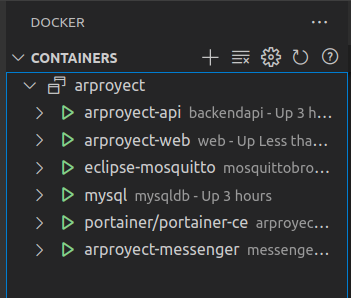
\includegraphics[scale=.60]{./Figures/docker-interfaz.png}
	\caption{Contenedores de Docker.}
	\label{fig:docker-interfaz}
\end{figure}

\section{Implementación de Hardware}
\label{sec:implementacionhw}

A continuación se describe la implementación del \textit{hardware} utilizado y detallado en el capítulo \ref{sec:hardware}.

Para el manejo de la red local se configuró un \textit{router} con una red Wi-Fi con filtrado de MAC Address y un servidor DHCP con entrega IP fija a los dispositivos del sistema.

En la figura \ref{fig:diagramared} podemos observar el diagrama de red del sistema, detallando que tipo de conexión realiza cada dispositivo.

\begin{figure}[H]
	\centering
	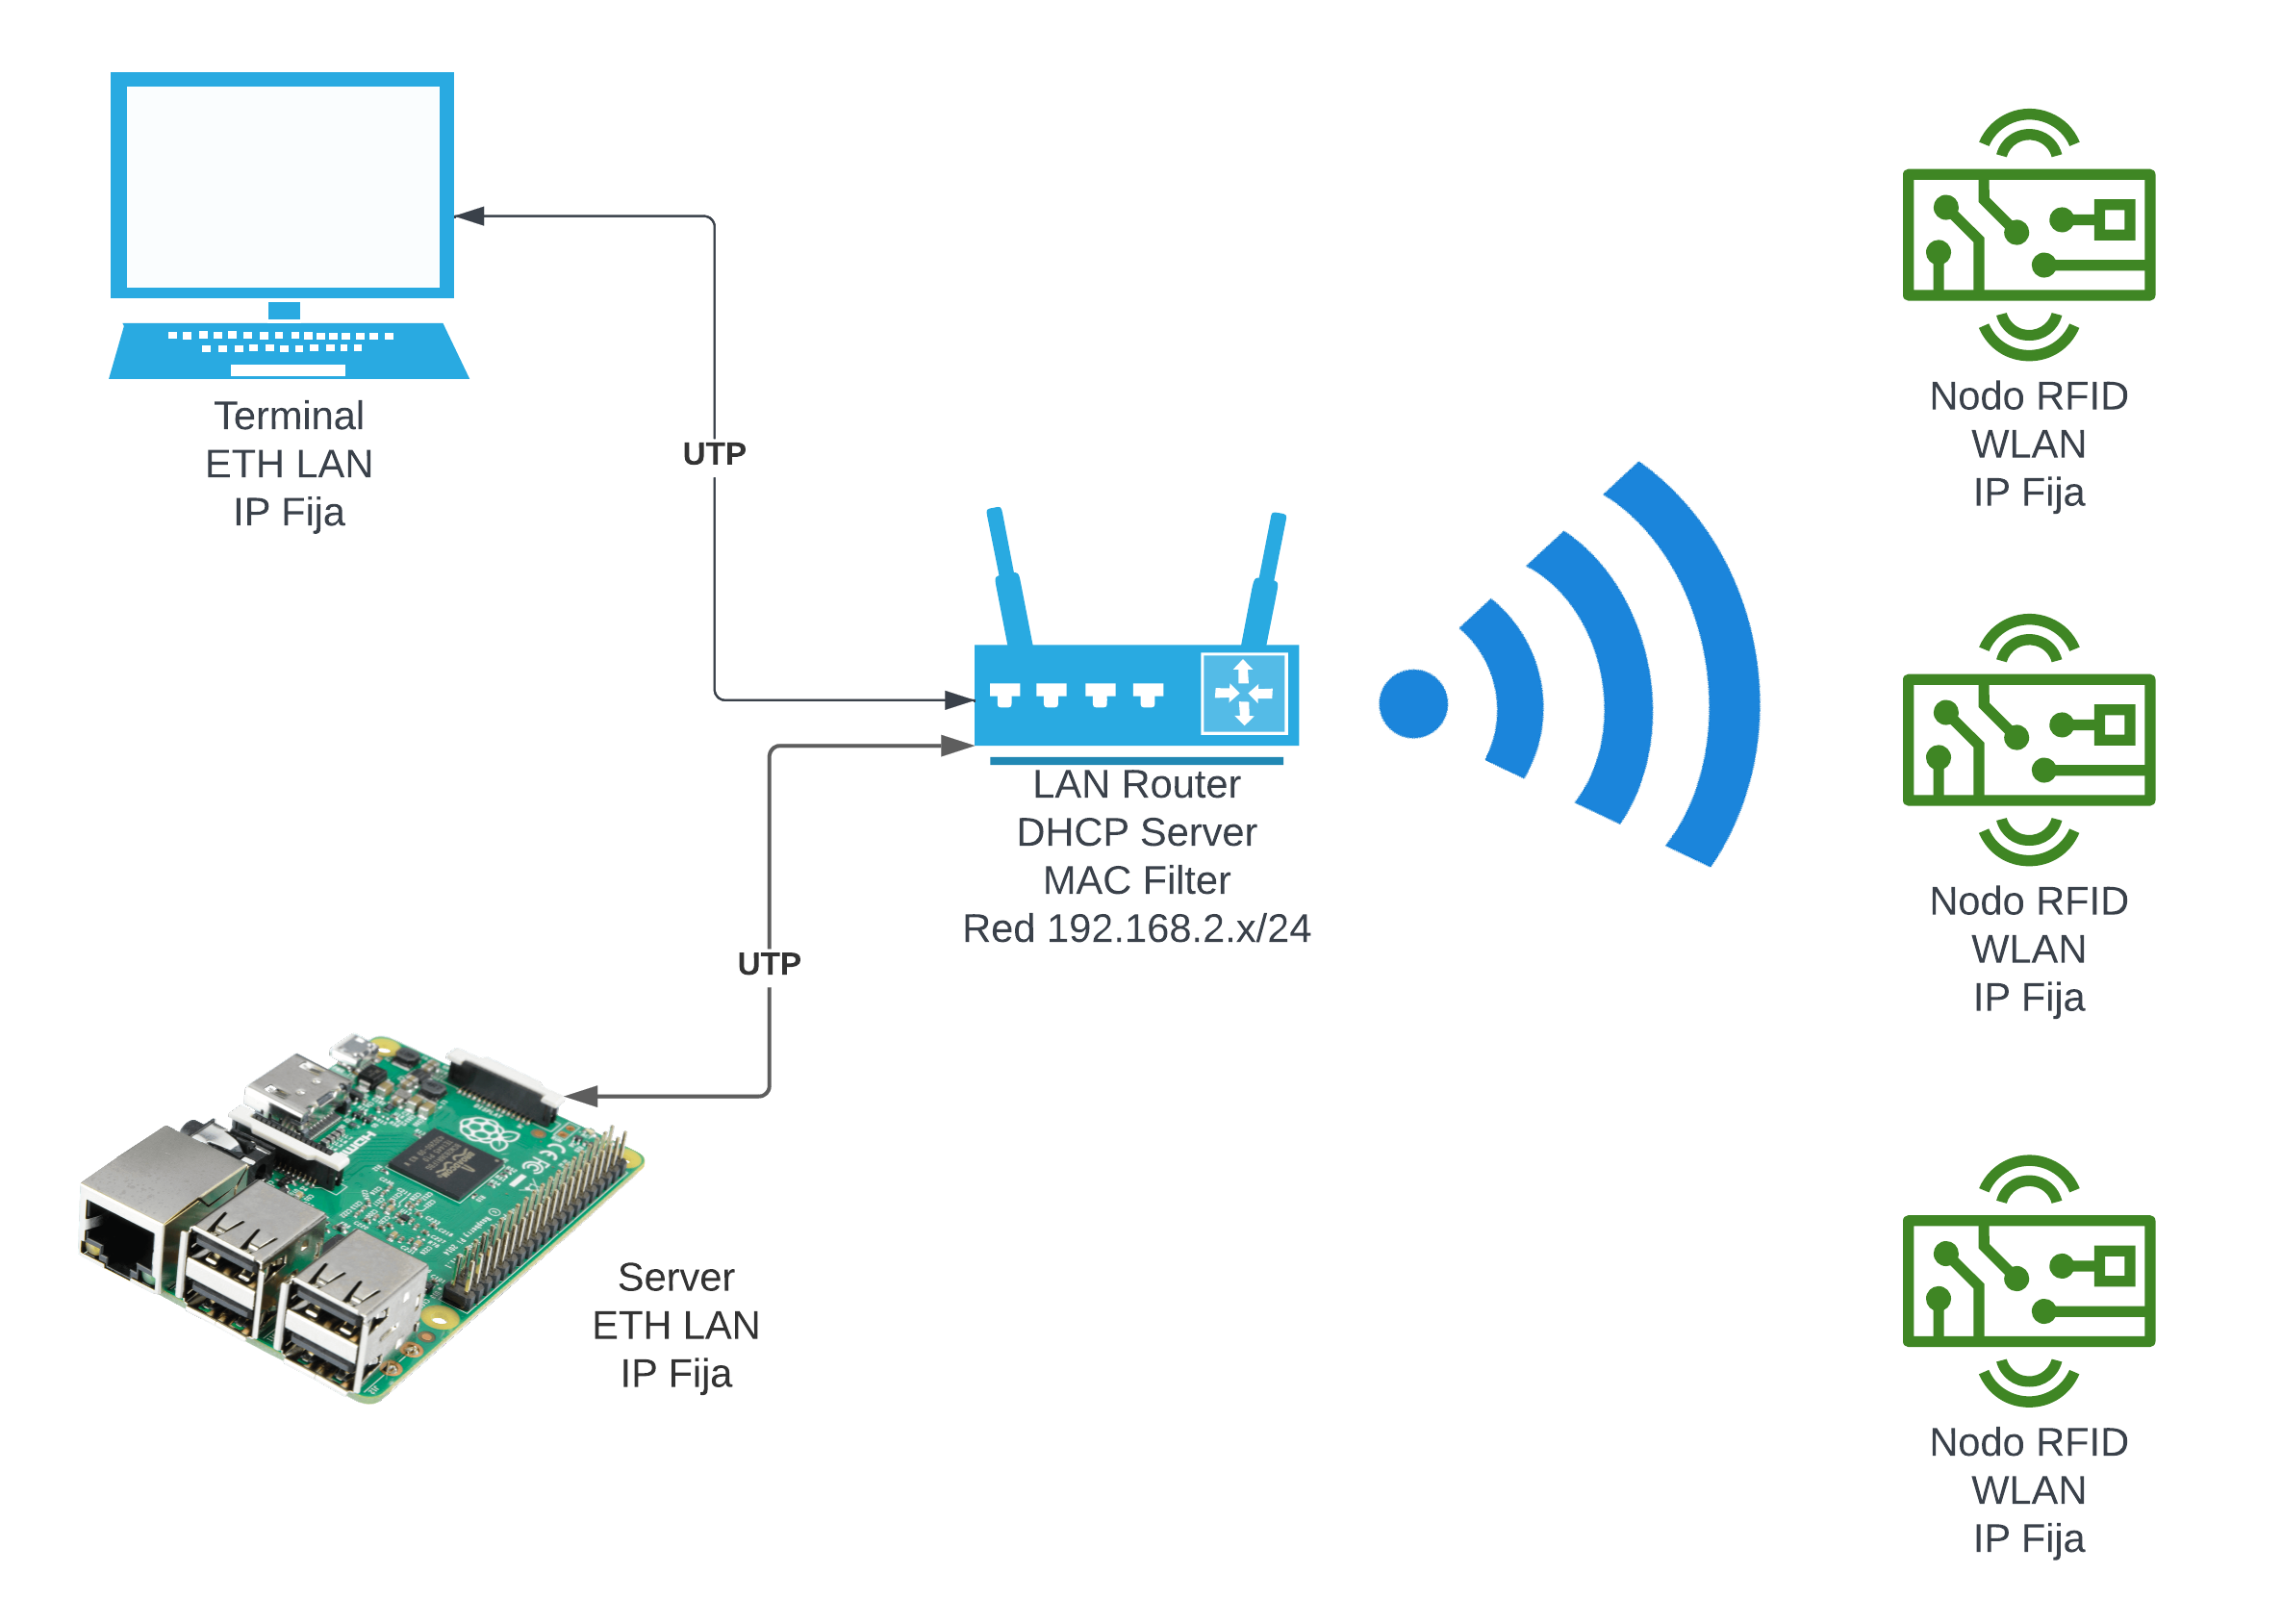
\includegraphics[scale=.10]{./Figures/diagrama-red.png}
	\caption{Diagrama de red del sistema.}
	\label{fig:diagramared}
\end{figure}

En el servidor se implementó una placa Raspberry Pi 4. Para esta placa se imprimió un gabinete personalizado utilizando una impresora de tipo 3D, se incluyó además un espacio adicional en el gabinete para agregar un disco tipo SSD para ampliar las capacidades de la placa.


Para los nodos se utilizó el microcontrolador NodeMCU Esp32, el sensor de radiofrecuenta MRC522 y un buzzer sonoro. El diseño del circuito en un \textit{software} especializado y la impresión de la placa PCB estuvo a cargo de colaboradores.  

Para realizar el \textit{build} o compilación del código fuente en el microcontrolador NodeMCU ESP32 se utilizó el \textit{framework} PlatformIO y el IDE Visual Studio Code (VSCODE).

En la figura \ref{fig:platformio-build} podemos observar el resultado de realizar el \textit{build}  o compilación del código fuente en la ESP32 utilizando PlatformIO y VSCode.

\begin{figure}[H]
	\centering
	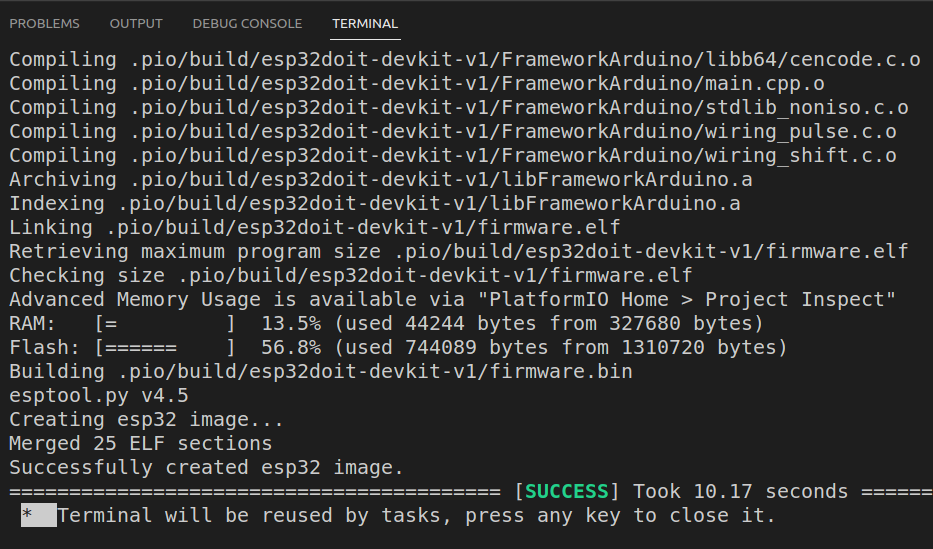
\includegraphics[width=\textwidth]{./Figures/platformio-build.png}
	\caption{Build en PlatformIO.}
	\label{fig:platformio-build}
\end{figure}

En la figura \ref{fig:platformio-upload} podemos observar el resultado de realizar el \textit{upload} o el copiado del código ya compilado a la ESP32 en PlatformIO. Además se detalla la instalación de las librerías que se utilizan en el proyecto.

\begin{figure}[H]
	\centering
	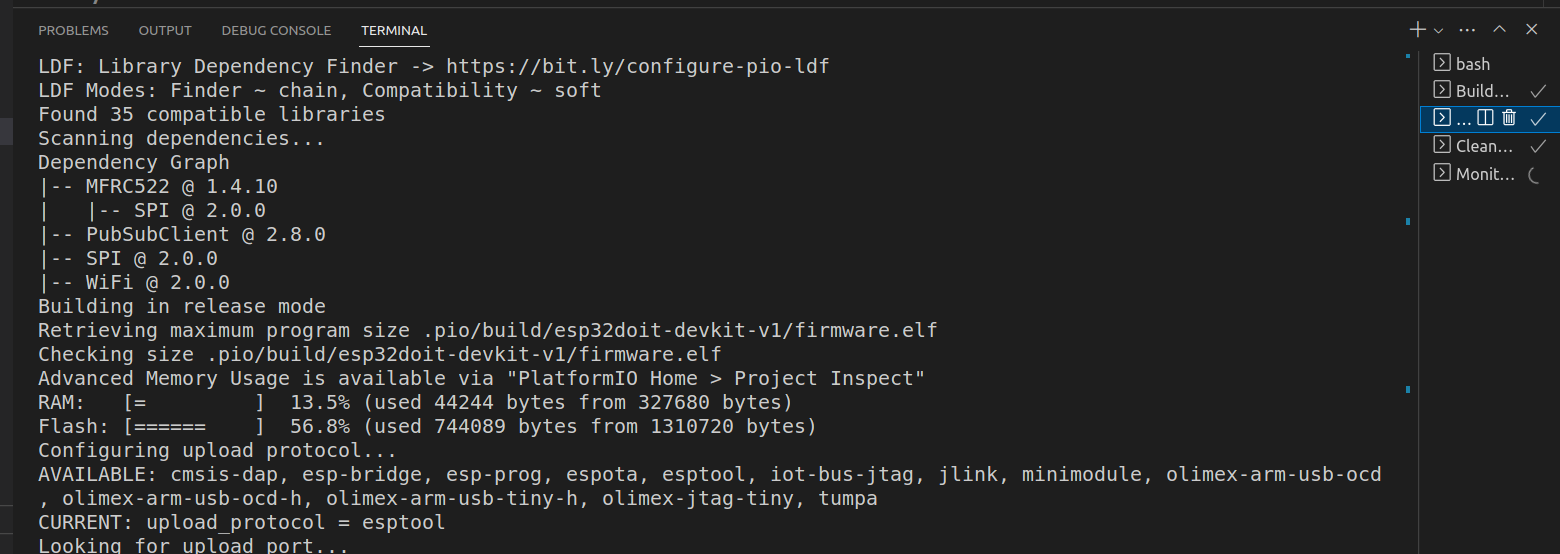
\includegraphics[width=\textwidth]{./Figures/platformio-upload.png}
	\caption{Upload en PlatformIO.}
	\label{fig:platformio-upload}
\end{figure}

Finalmente, en la figura \ref{fig:platformio-connect} podemos observar el resultado del código fuente ejecutándose en el microcontrolador y los detalles de la conexión exitosa a la red Wi-Fi y al \textit{broker} MQTT, indicando las direcciones IP y los puertos de conexión, además se muestran los mensajes que se configuraron en el código como el nombre de usuario y del nodo, la dirección IP y MAC de la ESP32 y el tópico MQTT al cual está suscripto. Esto se realiza mediante el \textit{framework}
 PlatformIO en modo monitor y con la ESP32 conectado a la PC mediante un cable USB de datos.
 
\begin{figure}[H]
	\centering
	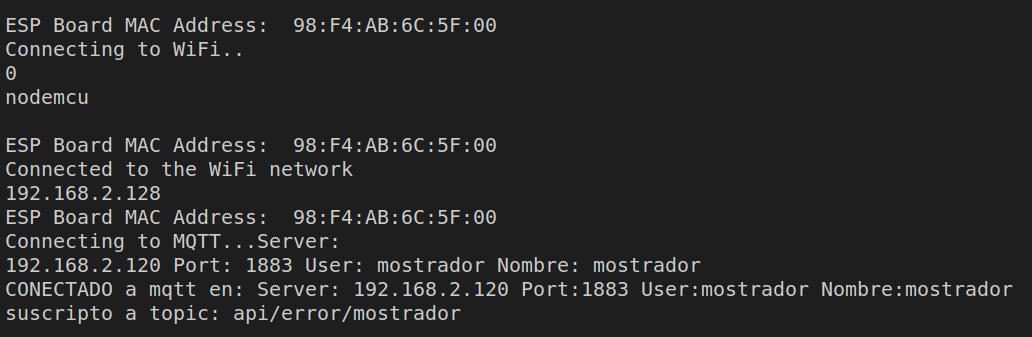
\includegraphics[width=\textwidth]{./Figures/platformio-connect.png}
	\caption{Upload en PlatformIO.}
	\label{fig:platformio-connect}
\end{figure}




% La idea de esta sección es resaltar los problemas encontrados, los criterios utilizados y la justificación de las decisiones que se hayan tomado.

% Se puede agregar código o pseudocódigo dentro de un entorno lstlisting con el siguiente código:

% \begin{verbatim}
% \begin{lstlisting}[caption= "un epígrafe descriptivo"]
% 	las líneas de código irían aquí...
% \end{lstlisting}
% \end{verbatim}

% A modo de ejemplo:

% \begin{lstlisting}[label=cod:vControl,caption=Pseudocódigo del lazo principal de control.]  % Start your code-block

% #define MAX_SENSOR_NUMBER 3
% #define MAX_ALARM_NUMBER  6
% #define MAX_ACTUATOR_NUMBER 6

% uint32_t sensorValue[MAX_SENSOR_NUMBER];		
% FunctionalState alarmControl[MAX_ALARM_NUMBER];	//ENABLE or DISABLE
% state_t alarmState[MAX_ALARM_NUMBER];						//ON or OFF
% state_t actuatorState[MAX_ACTUATOR_NUMBER];			//ON or OFF

% void vControl() {

% 	initGlobalVariables();
	
% 	period = 500 ms;
		
% 	while(1) {

% 		ticks = xTaskGetTickCount();
		
% 		updateSensors();
		
% 		updateAlarms();
		
% 		controlActuators();
		
% 		vTaskDelayUntil(&ticks, period);
% 	}
% }
% \end{lstlisting}



